\documentclass{article}


% if you need to pass options to natbib, use, e.g.:
%     \PassOptionsToPackage{numbers, compress}{natbib}
% before loading neurips_2025


% ready for submission
%\usepackage{neurips_2025}


% to compile a preprint version, e.g., for submission to arXiv, add add the
% [preprint] option:
%     \usepackage[preprint]{neurips_2025}


% to compile a camera-ready version, add the [final] option, e.g.:
\usepackage[final]{neurips_2025}


% to avoid loading the natbib package, add option nonatbib:
%    \usepackage[nonatbib]{neurips_2025}


\usepackage[utf8]{inputenc} % allow utf-8 input
\usepackage[T1]{fontenc}    % use 8-bit T1 fonts
\usepackage{hyperref}       % hyperlinks
\usepackage{url}            % simple URL typesetting
\usepackage{booktabs}       % professional-quality tables
\usepackage{amsfonts}       % blackboard math symbols
\usepackage{nicefrac}       % compact symbols for 1/2, etc.
\usepackage{microtype}      % microtypography
\usepackage{xcolor}         % colors


\usepackage{float}
\usepackage{graphicx}
%\usepackage{subcaption}
\usepackage{tablefootnote}

% For theorems and such
\usepackage{amsmath}
\usepackage{amssymb}
\usepackage{mathtools}
\usepackage{amsthm}

\usepackage{authblk}


%\usepackage{booktabs}
%\usepackage{caption}

\DeclareMathAlphabet{\mathbbold}{U}{bbold}{m}{n}
\newcommand{\bigbar}[1]{\overline{#1}}


%%%%%%%%%%%%%%%%%%%%%%%%%%%%%%%%%%%%%%%%%%%%%%%%%%%%%%%%%%%%%%%%%%%%%%%%%%%%%%%%%%%%%%%%%%%%%%%%%%%%

\bibliographystyle{plainnat}
%\bibliographystyle{abbrvnat}


\setcitestyle{authoryear,round,citesep={;},aysep={,},yysep={;}}

\title{REVE: A Foundation Model for EEG \\ Adapting to Any Setup with \\ Large-Scale Pretraining on 25,000 Subjects}

% The \author macro works with any number of authors. There are two commands
% used to separate the names and addresses of multiple authors: \And and \AND.
%
% Using \And between authors leaves it to LaTeX to determine where to break the
% lines. Using \AND forces a line break at that point. So, if LaTeX puts 3 of 4
% authors names on the first line, and the last on the second line, try using
% \AND instead of \And before the third author name.


% \author{%
%   David S.~Hippocampus \\
%   Department of Computer Science\\
%   Cranberry-Lemon University\\
%   Pittsburgh, PA 15213 \\
%   \texttt{hippo@cs.cranberry-lemon.edu} \\
%   % examples of more authors
%   % \And
%   % Coauthor \\
%   % Affiliation \\
%   % Address \\
%   % \texttt{email} \\
%   % \AND
%   % Coauthor \\
%   % Affiliation \\
%   % Address \\
%   % \texttt{email} \\
%   % \And
%   % Coauthor \\
%   % Affiliation \\
%   % Address \\
%   % \texttt{email} \\
%   % \And
%   % Coauthor \\
%   % Affiliation \\
%   % Address \\
%   % \texttt{email} \\
% }



\author{
Yassine El Ouahidi$^{1}$\thanks{Corresponding authors: \texttt{yassine.elouahidi@mistral.ai}, \texttt{giulia.lioi@imt-atlantique.fr}},
Jonathan Lys$^{1}$,
Philipp Thölke$^{2}$,
Nicolas Farrugia$^{1}$,\break
Bastien Pasdeloup$^{1}$,
Vincent Gripon$^{1}$,
Karim Jerbi$^{2, 3, 4}$,
Giulia Lioi$^{1*}$\\
\small $^{1}$ IMT Atlantique, Lab-STICC, UMR CNRS 6285, F-29238 Brest, France\\
\small $^{2}$ Psychology Department, Université de Montréal, Montreal, QC, Canada\\
\small $^{3}$ Mila (Quebec AI research institute), Montreal, QC, Canada\\
\small $^{4}$ UNIQUE (Quebec Neuro-AI research center), QC, Canada
}





% \affil[1]{Department of Computer Science, University A}
% \affil[2]{Department of Electrical Engineering, University B}


\begin{document}

%%%%%%%%%%%%%%%%%%%%%%%%%%%%

%%%%%%%%     TODO    %%%%%%%
%%%%%%%%     DONE    %%%%%%%

%%%%%%%% - (removed) %%%%%%%
%%%%%%%%   + (added) %%%%%%%

%%%%%%%%%%%%%%%%%%%%%%%%%%%%

\maketitle
% DONE: shortenned a bit (one sentence, see diff)
% https://www.diffchecker.com/18KbVDGc/

\begin{abstract}
Foundation models have transformed AI by reducing reliance on task-specific data through large-scale pretraining. While successful in language and vision, their adoption in EEG has lagged due to the heterogeneity of public datasets, which are collected under varying protocols, devices, and electrode configurations. Existing EEG foundation models struggle to generalize across these variations, often restricting pretraining to a single setup, resulting in suboptimal performance, in particular under linear probing.
We present REVE (Representation for EEG with Versatile Embeddings), a pretrained model explicitly designed to generalize across diverse EEG signals. REVE introduces a novel 4D positional encoding scheme that enables it to process signals of arbitrary length and electrode arrangement. Using a masked autoencoding objective, we pretrain REVE on over 60,000 hours of EEG data from 92 datasets spanning 25,000 subjects, representing the largest EEG pretraining effort to date.
REVE achieves state-of-the-art results on 10 downstream EEG tasks, including motor imagery classification, seizure detection, sleep staging, cognitive load estimation, and emotion recognition. With little to no fine-tuning, it demonstrates strong generalization, and nuanced spatio-temporal modeling. We release code, pretrained weights, and tutorials\footnote{ Project page: \url{https://brain-bzh.github.io/reve/}} to support standardized EEG research and accelerate progress in clinical neuroscience.
\end{abstract}



\section{Introduction} % DONE: modified the intro
\label{sec:introduction}

Electroencephalography (EEG) is a non-invasive technique widely used to study brain activity, with applications spanning brain-computer interfaces (BCIs), clinical diagnostics, and neuroscience research. 
% - 
% Despite its potential, EEG analysis remains fundamentally challenging due to the high variability in recording setups, electrode configurations, recording durations, and subject populations. 
%+
Despite its potential, the adoption of EEG-based technologies remains limited~\citep{lotte2018review}. A key challenge is developing models that generalize effectively to new subjects. EEG data varies widely in electrode configurations, recording conditions, and subject-specific factors, complicating model transferability. 
This heterogeneity has led to a fragmented ecosystem of datasets and task-specific models, many of which struggle to generalize across settings.

Foundation models have transformed natural language processing~\citep{achiam2023gpt4, dubey2024llama3, warner2024modernbert} and computer vision~\citep{radford2021learning, caron2021emerging, kirillov2023segment} by leveraging large-scale pretraining to enable transfer with minimal supervision. Their ability to produce general-purpose representations has sparked growing interest in building similar models for EEG~\citep{yang2024biot, wang2024cbramod, jiang2024labram, cui2024neuro, yuan2024brant2, wang2024eegpt}. Yet, EEG poses unique challenges including data heterogeneity, low signal-to-noise ratio, and the lack of standardized positional encoding to accommodate varying electrode configurations.

Recent EEG foundation models such as BIOT~\citep{yang2024biot}, Labram~\citep{jiang2024labram}, CBraMod~\citep{wang2024cbramod}, and NeuroGPT~\citep{cui2024neuro} adopt self-supervised learning (SSL) techniques for pretraining. While promising, many of these models rely solely on the TUH database~\citep{obeid2016temple} which uses a fixed 19 or 21-channel montage. As a result, they often fail to generalize to datasets with different electrode layouts or recording setups. Furthermore, existing positional encoding schemes, whether absolute~\citep{yang2024biot, jiang2024labram} or convolutional~\citep{wang2024cbramod}, lack the flexibility to accommodate spatial diversity, often necessitating full fine-tuning for transfer.

% - 
% In this work, we propose a foundation model for EEG that addresses these limitations and sets a new standard for scalability and generalization. Leveraging over 60,000 hours of data aggregated from 92 datasets encompassing 25,000 subjects, our work constitutes the most extensive EEG pretraining initiative to date. We employ a transformer-based spatio-temporal encoder-decoder architecture, trained via a masked autoencoder (MAE)~\cite{he2022masked} paradigm using modern SSL techniques. A key innovation of our approach is the introduction of a 4D positional encoding strategy, enabling the model to process EEG signals of arbitrary lengths and electrode configurations. This flexibility allows us to generate ready-to-use embeddings directly from raw EEG data, enabling seamless application to downstream tasks—a capability that defines our model, REVE, short for Representation for EEG with Versatile Embeddings.

% (old) 
% To overcome these challenges, we present REVE (Representation for EEG with Versatile Embeddings), a scalable foundation model for EEG. REVE is trained on over 60,000 hours of recordings from 92 datasets encompassing 25,000 subjects, the most extensive EEG pretraining effort to date. Our model employs a spatio-temporal transformer architecture trained via a masked autoencoder (MAE)~\cite{he2022masked} objective. A key innovation is a 4D positional encoding scheme that enables the model to process signals of varying lengths and electrode configurations, producing reusable embeddings that generalize across a wide range of downstream tasks.

To address the limitations in current EEG foundation models, we consider three core contributions that enable scalable, generalizable representation learning across diverse, large-scale EEG datasets. 

First, we propose a novel 4D positional encoding scheme that enables flexible modeling of EEG signals with varying temporal lengths and electrode configurations. Unlike existing absolute or convolutional encodings, our formulation naturally supports spatial and temporal variability, eliminating the need for fixed montages or fine-tuning of positional priors.

Thanks to this flexible positional encoding method, we are able to train with a wider range of EEG configurations, allowing to scale to larger and more heterogeneous datasets. To this end, we curate the largest and most diverse EEG corpus to date, comprising over 60,000 hours of data from 92 datasets and 25,000 subjects. This diverse collection spans clinical, BCI, and research domains, providing the scale and diversity necessary for robust pretraining.

% Collecting such a large dataset allows to introduce REVE, the 
Combining architectural flexibility with large-scale data results in REVE (Representation for EEG with Versatile Embeddings), a spatio-temporal transformer model trained with a modified masked autoencoder (MAE)~\citep{he2022masked} objective that promotes learning better representations in the model. REVE learns general-purpose EEG representations that transfer effectively across a wide range of downstream tasks.

% - 
% Our model achieves state-of-the-art performance across a diverse range of benchmarks, including BCI paradigms and clinical tasks, surpassing existing EEG foundation models in accuracy on key datasets. Additionally, scaling studies demonstrate performance improvements with larger model sizes, underscoring the potential of scalable pretraining for enhanced generalization across datasets and tasks. To promote accessibility and reproducibility, we provide open-source code, pretrained weights of various sizes, and tutorials to adapt the model to diverse EEG applications.

% - 
% By addressing the unique challenges of EEG analysis through large-scale pretraining, innovative encoding strategies, and modern training techniques, our work establishes a foundation for unifying EEG processing, driving advancements in BCIs, clinical diagnostics, and neuroscience.

% + 
REVE achieves state-of-the-art performance across numerous benchmarks, including BCI and clinical datasets, outperforming prior EEG foundation models. Our scaling studies further show improved generalization with larger model sizes, reinforcing the benefits of large-scale pretraining. To support adoption, we release open-source code, pretrained models of multiple sizes, and detailed tutorials for applying REVE to various EEG tasks. By addressing the unique challenges of EEG with scalable architectures and flexible spatial encoding, REVE establishes a unified foundation for EEG analysis and paves the way for new advances in neuroscience and clinical applications.

\section{Methods}
\label{sec:method}


\begin{figure}[h]
\centering
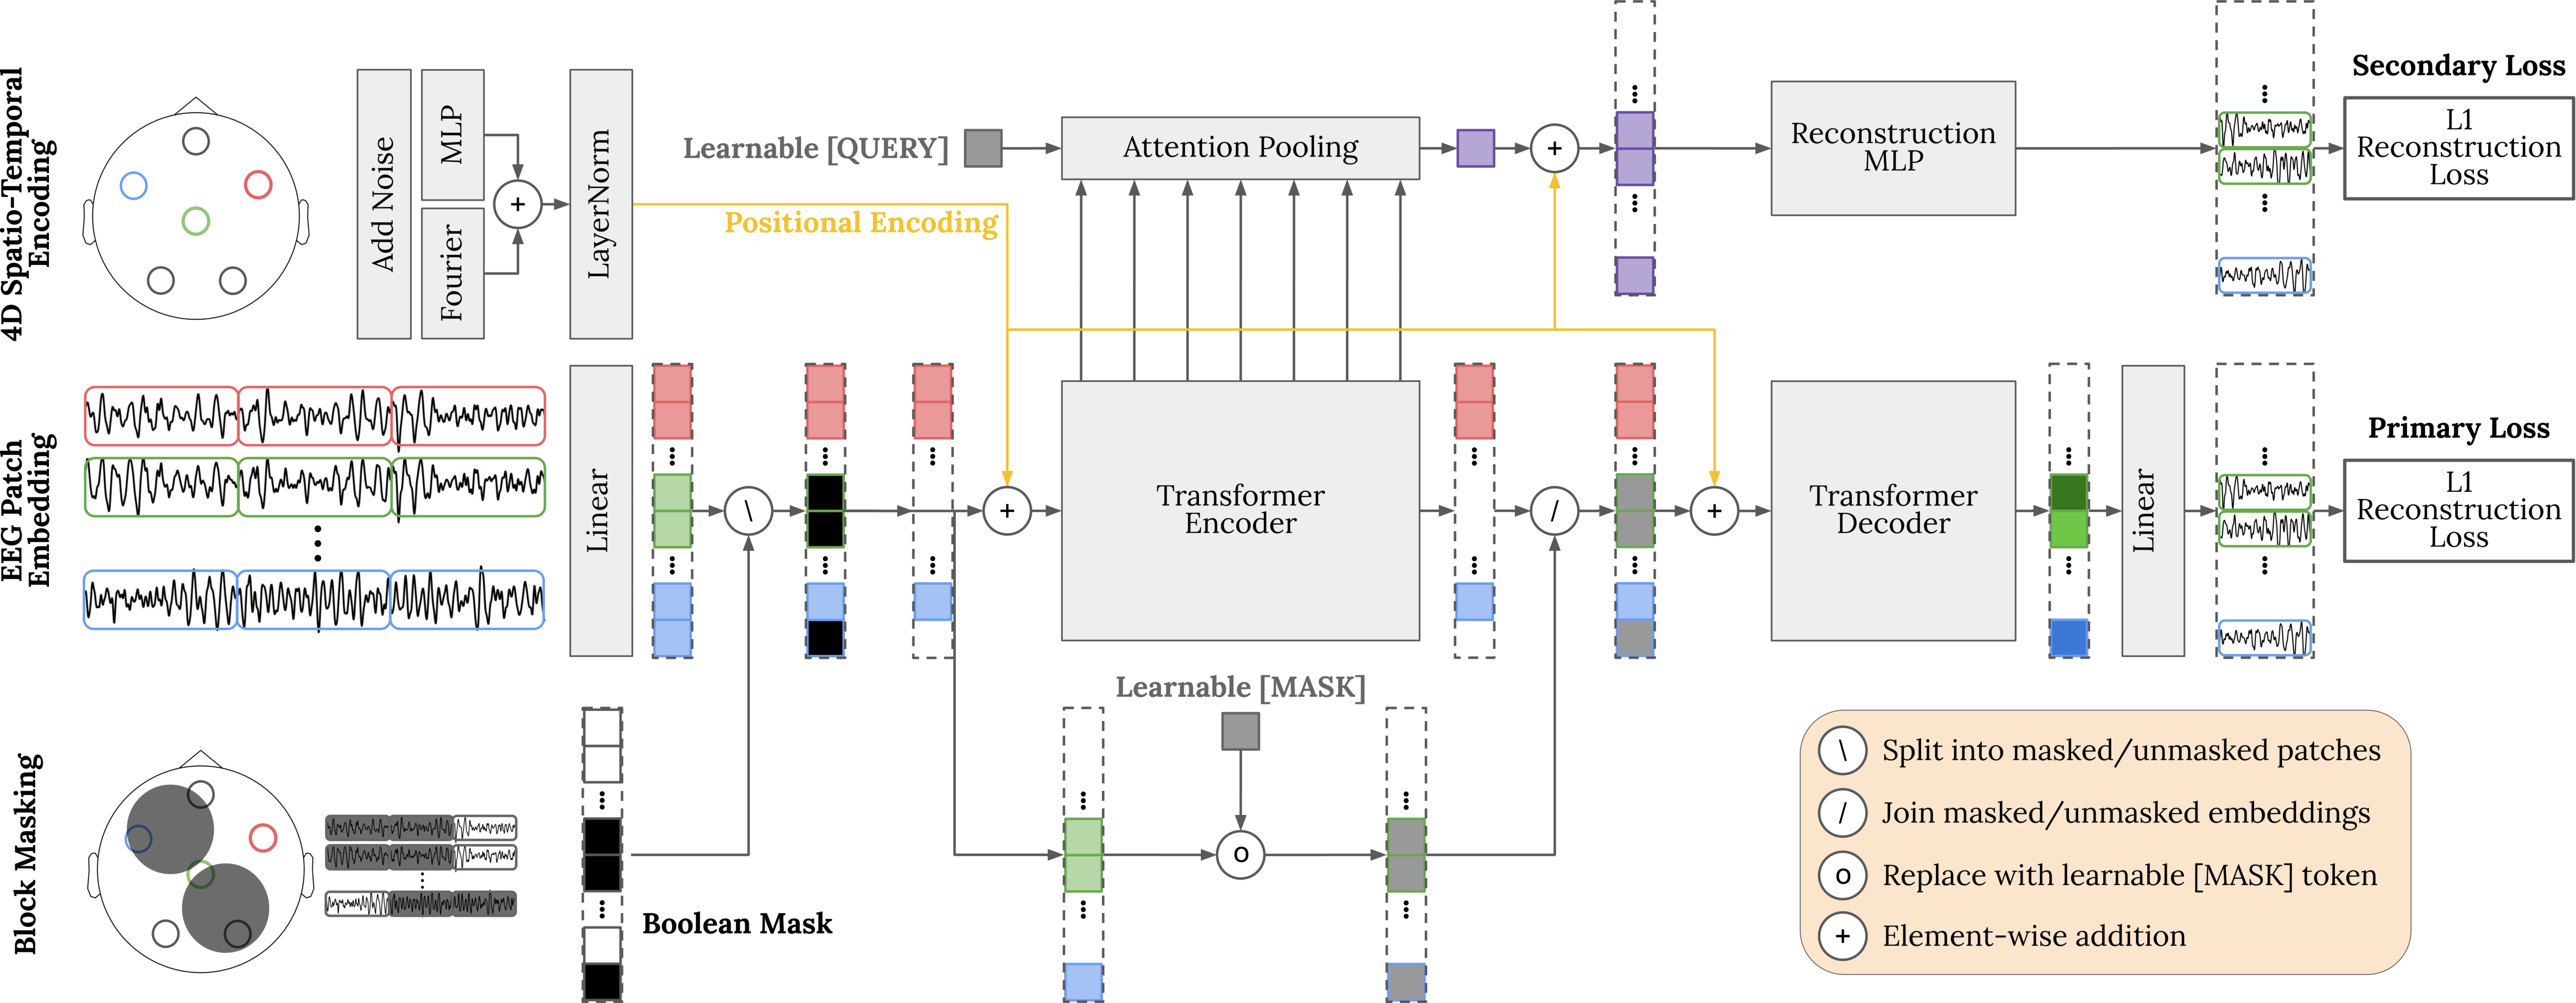
\includegraphics[width=.92\linewidth]{figures/figure_REVE.pdf}
\caption{Overview of the \textbf{REVE} pretraining framework. The model processes multi-channel EEG data through a linear \textbf{Patch Embedding} where signals are divided into overlapping temporal patches for each channel and embedded with a linear layer. \textbf{4D Spatio-Temporal Position Encoding} combines spatial coordinates of electrodes with temporal patch indices, augmented with noise for robust generalization. A \textbf{Block Masking Strategy} masks contiguous regions across spatial and temporal dimensions to simulate realistic disruptions. The transformer encoder processes unmasked embeddings. Updated embeddings are joined with learnable placeholders for the masked tokens, from which raw EEG is reconstructed using the decoder. The \textbf{Primary Task} predicts raw EEG signals directly, while the \textbf{Secondary Task} trains a single global token via attention pooling to summarize the input. Both tasks minimize an $\text{L}_1$    reconstruction loss.}

% - 
% Overview of the \textbf{REVE} architecture along its pretraining framework. The model processes multi-channel EEG data, starting with \textbf{EEG Patch Embedding}, where signals are divided into overlapping temporal patches for each channel and linearly embedded. \textbf{4D Spatio-Temporal Position Encoding} combines spatial coordinates of electrodes with temporal patch indices, augmented with noise for robust generalization. A \textbf{Block Masking Strategy} masks contiguous regions across spatial and temporal dimensions to simulate realistic disruptions. The transformer encoder processes unmasked embeddings. Updated embeddings are joined with learnable placeholders for the masked tokens, from which raw EEG is reconstructed using the decoder. The \textbf{Primary Task} predicts raw EEG signals directly, while the \textbf{Secondary Task} trains a single global token via attention pooling to summarize the input. Both tasks minimize an $L_1$ reconstruction loss.
\label{fig:archi}
\end{figure}
% +
We pretrain our encoder using a masked autoencoder objective. The REVE encoder consists of a patch embedding module, a 4D position encoding module, and a transformer backbone. During pretraining, we apply spatio-temporal contiguous masking to the patch embeddings and jointly train the encoder and decoder to reconstruct the missing segments of EEG, enabling the encoder to learn robust feature representations. Subsequent hyperparameter values are listed in Table~\ref{tab:summary} in the Appendix.

\subsection{EEG Representation and Block Masking strategy}
% DONE: merged the 2 shortened sub-sections
\label{subsec:patching}
\label{subsec:mask-strat}

% - We represent multi-channel EEG data as \(\mathbf{X} \in \mathbb{R}^{C \times T}\), where \(C\) is the number of EEG channels/electrodes and \(T\) is the number of time samples. Electrode positions are denoted as \(\mathbf{P} \in \mathbb{R}^{C \times 3}\), corresponding to 3D points \((x, y, z)\) in a coordinate system relative to the head. To process the data, we segment each EEG channel into \(p\) patches using a window of size \(w\) samples and an overlap of \(o\) samples, following the approach proposed in BIOT~\cite{yang2024biot}. We do not use padding and discard incomplete patches. As a result, \(\mathbf{X}\) becomes \(\mathbf{Xp} \in \mathbb{R}^{C \times p \times w}\) where $p = \left\lceil \frac{T - w}{w - o} \right\rceil + \mathbbold{1} \left[ (T - w) \bmod (w - o) \neq 0 \right]$. We then embed each patch using a linear layer, transforming \(\mathbf{Xp}\) into \(\mathbf{E} \in \mathbb{R}^{C \times p \times D_E}\), where $D_E$ is the embedding dimension.

% +
We represent multi-channel EEG data as $\mathbf{X} \in \mathbb{R}^{C \times T}$, where $C$ is the number of electrodes and $T$ the number of time samples, electrode positions are given by $\mathbf{P} \in \mathbb{R}^{C \times 3}$, corresponding to their 3D coordinates. To process the data, we segment each channel into patches of size $w$ with overlap $o$, following BIOT~\citep{yang2024biot}. This yields $p = \left\lceil \frac{T - w}{w - o} \right\rceil + \mathbbold{1} \left[ (T - w) \bmod (w - o) \neq 0 \right]$ non-overlapping patches (discarding any incomplete ones), and reshapes $\mathbf{X}$ into $\mathbf{Xp} \in \mathbb{R}^{C \times p \times w}$. Each patch is linearly embedded, resulting in $\mathbf{E} \in \mathbb{R}^{C \times p \times D_E}$, where $D_E$ is the embedding dimension.


% Our methodology introduces a novel block masking strategy, combining spatial and temporal dimensions to effectively mask EEG data for our pretraining routine. While spatial blocks have already proven to be useful in EEG~\cite{mohammadi2024eeg2rep,  guetschel2024s}, we extend this principle into the temporal dimension. This leverages findings from image processing and EEG signal analysis, which suggest that structured masking outperforms random masking~\cite{xie2022simmim}. We confirm this phenomenon in Table~\ref{tab:rmask_results} in the Appendix. As neighboring segments of EEG, in both spatial and temporal domain, are typically similar, the challenge of signal reconstruction is greatly reduced with inadequate masking strategies. Uniformly random masking of patches, for example, may leave redundant information exposed, while block masking efficiently disrupts spatial and temporal patterns.

% +
To enhance learning during pretraining, we apply a joint spatio-temporal block masking strategy that masks structured regions across both spatial and temporal dimensions. Random masking, proposed for EEG by~\citet{chien2022maeeg}, was later improved through spatial masking~\citep{mohammadi2024eeg2rep, guetschel2024s}.  In this work, we extend the masking strategy to the temporal domain. This builds on insights from image modeling, where structured masking outperforms random masking~\citep{xie2022simmim}, a trend also supported by our ablation results (Table~\ref{tab:rmask_results}, Appendix). As neighboring segments of EEG, in both spatial and temporal domain, are typically similar, naive random masking could leave redundant information exposed, reducing the difficulty of reconstruction. In contrast, block masking better disrupts these patterns, encouraging more effective learning.

% - Our block masking strategy is defined by the following parameters: \textbf{Masking Ratio} (\(M_r\)) determines the proportion of tokens to be masked. \textbf{Spatial Masking Radius} (\(R_s\)) specifies a masking radius around a given channel. \textbf{Temporal Masking Radius} (\(R_t\)) defines the time range around each masked token to include in the masked region. \textbf{Dropout Ratio} (\(D_r\)) indicates the proportion of masked tokens where the entire time-series of the corresponding channel is dropped. \textbf{Dropout Radius} (\(R_d\)) determines the spatial extent around the central channel for grouping tokens affected by dropout. For tokens not included in the dropout, \textbf{Combined Masking Strategy} applies temporal masking within radius \(R_t\). At this step, we obtain a set a binary mask $\mathbf{B} \in \mathbb{R}^{C \times p}$ with $N_{\text{m}} = \lfloor (1 - M_r) \cdot C \cdot p \rfloor$ zeros for the masked entries and $N_{\bigbar{\text{m}}} = C\cdot p - N_{\text{m}}$ ones for the non-masked entries.

% +
Our block masking strategy is governed by the following parameters: The masking Ratio $M_r$ controls the overall proportion of masked tokens. The spatial Masking Radius $R_s$ and Temporal Masking Radius $R_t$ respectively define the spatial extent (around a selected channel) and the time window (around a selected token) to be masked. Similarly, the Dropout Ratio $D_r$ sets the fraction of masked tokens for which the entire time series of the corresponding channel is dropped, while the dropout Radius $R_d$ determines the spatial neighborhood affected by dropout. For tokens not dropped, temporal masking is applied within radius $R_t$. This process yields a binary mask $\mathbf{B} \in \mathbb{R}^{C \times p}$, containing $N_{\text{m}} = \lfloor (1 - M_r) \cdot C \cdot p \rfloor$ masked entries (zeros) and $N_{\bar{\text{m}}} = C \cdot p - N_{\text{m}}$ unmasked entries (ones).

\subsection{4D Position Encoding Strategy}
\label{subsec:fourier}
% - 
% Unlike previous studies that relied on fixed-sized learned embeddings, our model allows for EEG signals of any duration or configuration. It generates position encoding relative to spatio-temporal coordinates of the tokens to produce a flexible encoding strategy that generalizes well to unseen setups.

% +
Unlike prior works that rely on learned embedding tables for spatial encoding vectors~\citep{jiang2024labram, wang2024cbramod}, we directly generate position encodings from the spatio-temporal coordinates of the tokens, allowing the processing of signals of any length or EEG layout and enabling better generalization to unseen setups. More specifically, our method uses a transformation applicable to each position, utilizing the actual 3D coordinates and timestep of each EEG patch, enabling the model to handle arbitrary electrode configurations and sequence lengths without relying on learned embeddings.
% TODO: include ref to ablation on learnable vs fixed

\paragraph{4D Positional Encoding and Spatial Augmentation.}
% DONE: shorten
We start with the spatial positions of the EEG electrodes $\mathbf{P} \in \mathbb{R}^{C \times 3}$, where each row of \(\mathbf{P}\) contains the \((x, y, z)\) coordinates of a channel, to which we add Gaussian noise with standard deviation \(\sigma_{\text{noise}}\). This improves generalization to diverse electrode positions and ensures robustness to variability in head size or electrode placement. We extend $\mathbf{P}$ with a temporal component, resulting in $\mathbf{P}_{\text{ext}} \in \mathbb{R}^{C \times p \times 4}$,
where $p$ is the number of patches obtained from segmenting EEG signal, as defined in Section~\ref{subsec:patching}. The temporal dimension is represented as discrete values from \(1\) to \(p\), scaled by a factor $s_{\text{t}}$ to ensure a scale similar to the spatial dimensions.

\paragraph{4D Fourier-Based Position Encoding.}

% DONE: shorten
Building on the 2D approach proposed by~\citet{defossez2023decoding}, we extend the Fourier positional encoding method to 4D in our encoding strategy, as follows. Each positional component $(x,y,z,t)$ of $\mathbf{P}_{\text{ext}}$ is projected into a multi-frequency space, using $n_{\text{freq}}$ frequencies per dimension. The frequency assignment follows a Cartesian product structure, \emph{i.e.}, all combinations of frequencies across the four dimensions contribute to the encoding, resulting in a flattened vector of dimension $n_{\text{freq}}^4$.
A hierarchical periodicity emerges: the period of $x$ is $n_{\text{freq}}^1$, of $y$ is $n_{\text{freq}}^2$, of $z$ is $n_{\text{freq}}^3$, and of $t$ is $n_{\text{freq}}^4$. Then, applying sine and cosine transformations doubles the embedding size, producing a positional vector of dimension $2\cdot n_{\text{freq}}^4$. We ensure that the  embedding dimension matches the hidden size required by the 4DPE module, with $n_{\text{freq}} \in \{3, 4, 5\}$ resulting in the final embedding $\mathbf{F}_{\text{pe}} \in \mathbb{R}^{C \times p \times D_E}$. The 4D encoding adds minimal compute overhead, with sinusoidal computations and a small linear layer. Computational cost scales linearly with the number of input tokens (channels $\times$ temporal patches) and is negligible relative to the transformer backbone.


% - 
% \paragraph{Learnable Encoding Adjustment}
% In parallel, we process \(\mathbf{P}_{\text{ext}}\) through a linear layer followed by a GELU activation~\cite{hendrycks2016gaussian}, and LayerNorm~\cite{lei2016layernorm}, yielding $\mathbf{F}_{\text{lin}} \in \mathbb{R}^{C \times p \times D_E}$. This learnable component adjusts the fixed Fourier encoding, adapting it to the specific dataset and task. It can also account for possible dimension truncation previously described.

% \paragraph{Final Position Encoding}
% The resulting vector is: $\mathbf{P}_{\text{enc}}=\text{LayerNorm}(\mathbf{F}_{\text{pe}} + \mathbf{F}_{\text{lin}})$ with \(\mathbf{P}_{\text{enc}} \in \mathbb{R}^{C \times p \times D_E}\). The Fourier encoding serves as the primary mechanism for capturing spatio-temporal structure, while the linear layer ensures adaptability to variations, such as tasks with electrodes in non-standard locations. This final positional encoding is added to the (non-masked) patch embeddings before going into the transformer encoder, similarly to MAE~\cite{he2022masked} and following absolute positional encoding~\cite{vaswani2017attention} practices. 


% +
\paragraph{Final Adjusted Position Encoding.}
To complement the fixed Fourier features, we also process $\mathbf{P}_{\text{ext}}$ through a linear layer followed by GELU~\citep{hendrycks2016gaussian} and LayerNorm~\citep{lei2016layernorm}, producing a learnable representation $\mathbf{F}_{\text{lin}} \in \mathbb{R}^{C \times p \times D_E}$. This component adapts the positional encoding to the specific dataset and task, and can compensate for any truncation in the Fourier basis. The final positional encoding is given by $\mathbf{P}_{\text{enc}} = \text{LayerNorm}(\mathbf{F}_{\text{pe}} + \mathbf{F}_{\text{lin}})$, combining the structured inductive bias of Fourier features with the flexibility of learned adaptation. This vector is added to the non-masked patch embeddings before being passed to the transformer encoder similarly to MAE~\citep{he2022masked}, and is consistent with standard absolute positional encoding practices~\citep{vaswani2017attention}. The ablation study in Table~\ref{tab:ablation_pe} confirms that this method outperforms both fixed learnable and purely MLP-based positional encoding schemes.

\subsection{Transformer}
\label{subsec:transfo}
% - 
% Our model builds upon the standard transformer architecture~\cite{vaswani2017attention} by integrating several modern improvements to enhance efficiency, stability, and performance.

% \paragraph{Normalization and Activation.} We replace LayerNorm with RMSNorm~\cite{zhang2019root} for better training stability, and choose GEGLU~\cite{shazeer2020glu} as the activation function in feed-forward layers. GEGLU has shown to outperform standard GELU across various transformer-based architectures through more expressive gating mechanisms~\cite{geiping2023cramming, warner2024modernbert}.

% \paragraph{Feed-Forward Network (FFN) Design.} Our FFN layers follow a two-layer structure with an expansion ratio of \( \frac{8}{3} \), aligning with best practices from state-of-the-art foundation models such as LLaMA~\cite{touvron2023llama1, touvron2023llama2}, ModernBERT~\cite{warner2024modernbert}, Qwen~\cite{bai2023qwen} or Mistral~\cite{jiang2023mistral}. The GLU-based FFN layers are then expanded by a ratio of 2 (\(2 \cdot \frac{8}{3}\) embedding dimension).

% \paragraph{No Bias Terms.} Following~\citet{warner2024modernbert}, we remove bias terms from all linear layers except the final decoder layer and LayerNorm. This reallocates the parameter budget to linear transformations, improving efficiency.

% \paragraph{Flash Attention v2.} We use Flash Attention v2~\cite{dao2022flashattention, dao2023flashattention2} for memory and computational efficiency in the attention. This kernel reduces the softmax computation overhead and ensures scalability for large sequences, while preserving theoretical foundations of the transformer.

% DONE: shorten
% +
Our model extends the standard Transformer architecture~\citep{vaswani2017attention} with enhancements that improve efficiency and stability.
We use RMSNorm~\citep{zhang2019root} in lieu of LayerNorm as a \textbf{normalization layer} for better training stability, and choose GEGLU~\citep{shazeer2020glu} as the \textbf{activation} function in the feed-forward network (FFN) layers as it outperforms standard GELU through more expressive gating mechanisms~\citep{geiping2023cramming}. This choice is further supported by the ablation results in Table~\ref{tab:ablation_activation}.
Our \textbf{FFN layers} follow a two-layer structure with an expansion ratio of \( \frac{8}{3} \), consistent with designs from LLaMA~\citep{touvron2023llama1}, Qwen~\citep{bai2023qwen} or Mistral~\citep{jiang2023mistral}.
Following~\citet{Dayma_DALLE_Mini_2021}, we \textbf{remove bias terms} from all linear layers except the final decoder layer. This reallocates the parameter budget to linear transformations, improving efficiency. We use \textbf{Flash Attention v2}~\citep{ dao2023flashattention2} for memory and computational efficiency in the attention as it reduces the softmax overhead and ensures scalability to long sequences, while maintaining the core transformer formulation. 

\subsection{Masked EEG Reconstruction Methodology}
% DONE: shorten and simplify

% - 
% During pretraining, our model reconstructs the raw EEG signal of masked patches using information from the visible (unmasked) patches. Let the set of masked patches be denoted as $\mathbf{P}_{\text{m}} \in \mathbb{R}^{N_{\text{m}}\times w}$, and the set of visible patches as $\mathbf{P}_{\bigbar{\text{m}}} \in \mathbb{R}^{N_{\bigbar{\text{m}}} \times w}$, with $N_{\text{m}}$ and $N_{\bigbar{\text{m}}}$ as defined in Section \ref{subsec:mask-strat}. The associated patch embeddings are denoted as $\mathbf{E_m}$ for masked patches and  $\mathbf{E_{\bigbar{m}}}$ for visible patches.

% +
During pretraining, our model reconstructs EEG signal of masked patches using information from the visible, unmasked patches. The overall pretraining framework is illustrated in Figure~\ref{fig:archi}. 

Let $\mathbf{P}_{\text{m}} \in \mathbb{R}^{N_{\text{m}}\times w}$, and $\mathbf{P}_{\bigbar{\text{m}}} \in \mathbb{R}^{N_{\bigbar{\text{m}}} \times w}$ denote the masked and visible patches, respectively, with $N_{\text{m}}$ and $N_{\bigbar{\text{m}}}$ as defined in Section \ref{subsec:mask-strat}. The associated patch embeddings are denoted as $\mathbf{E_m}$ for masked patches and  $\mathbf{E_{\bigbar{m}}}$ for visible patches.

% - 
% The Masked AutoEncoder (MAE) structure used for reconstruction is based on the original design proposed in~\citet{he2022masked}. Both the encoder and decoder adopt the Transformer architecture described in Section \ref{subsec:transfo}. As in the original MAE, the encoder is designed to be larger than the decoder.

% + 
We adopt the MAE structure from~\citet{he2022masked}, with a larger encoder and a lighter decoder each following the architecture described in Section~\ref{subsec:transfo}. Only the embeddings of the visible patches $\mathbf{E}_{\bigbar{\text{m}}}$, enriched with their positional encodings are passed through the encoder, to produce latent representations $\mathbf{F}_{\bigbar{\text{m}}}$. 
Masked patches are represented using a learned embedding, repeated $N_{\text{m}}$ times and also augmented with positional encodings.
Before entering the decoder, positional encodings are re-added to both visible and masked latent patches. Together, they form the decoder input from which the raw EEG signal of the masked patches is reconstructed.

Unlike the original MAE, which uses a separate set of fixed positional encodings for the decoder, we reuse the same encoding for both the encoder and decoder. This design ensures flexibility for processing EEG signals with varying temporal lengths and electrode configurations.

The output of the decoder transformer, is passed through a linear projection layer that maps latent patches back into the signal space, reconstructing the raw EEG signal of the masked patches. Reconstructed patches minimize the $\text{L}_1$ loss relative to the original raw EEG patches:
\begin{equation}
    \mathcal{L} = \frac{1}{|\mathbf{P}_{\text{m}}|} \sum_{i \in \mathbf{P}_{\text{m}}} \left\lVert \mathbf{\hat{P}}_{\text{m}}^{(i)} -\mathbf{P}_{\text{m}}^{(i)} \right\rVert_1
\end{equation}
where $\mathbf{\hat{P}}_{\text{m}}^{(i)}$ represents the reconstructed signal for patch $i$, and $\mathbf{P}_{\text{m}}^{(i)}$ is the original signal. We chose $\text{L}_1$ loss over $\text{L}_2$ due to the inherently noisy nature of EEG signals. While $\text{L}_2$ amplifies the influence of noise, $\text{L}_1$ loss offers greater robustness by reducing the impact of outliers.

% - 
% In addition to the primary reconstruction loss, we introduce a second reconstruction task, which is also a novel contribution. In addition to reconstructing the raw signal directly from the encoded tokens, we use a single token and perform attention pooling across the outputs of all Multi-Head Attention (MHA) layers in the encoder. Specifically, we extract the output tokens from each MHA block (post-FFN), concatenate them, and use these as keys and values. A learned query token attends to these concatenated outputs, producing an attention-pooled representation of all tokens. This single token is then repeated to match the number of masked tokens, with positional encoding added for each masked token. Finally, a 2-layer FFN reconstructs the raw signal for each masked patch. Similarly to the primary loss, we use $L_1$ loss to compare the reconstructed patches to the original raw EEG patches. The final loss is a weighted sum (with parameter $\lambda$) of the two: $\text{Loss} = \text{Primary Loss} + \lambda \cdot \text{Secondary Loss}$

%+
In addition to the main reconstruction loss, we introduce a secondary task that reconstructs masked patches from a compact global representation. We apply attention pooling over the outputs of all Multi-Head Attention (MHA) layers in the encoder: the output tokens (after FFN) from each MHA block are concatenated and attended by a learned query token. This pooled token is then repeated, enriched with positional encodings, and passed through a 2-layer FFN to reconstruct the masked patches. As with the primary loss, we use $\text{L}_1$ loss for reconstruction. The total loss is a weighted sum: $\text{Loss} = \text{Primary Loss} + \lambda \cdot \text{Secondary Loss}$

This secondary loss encourages the encoder to distribute useful information across all layers, mitigating over-specialization in the final layer and yielding more generalizable representations.

% -
% The secondary loss addresses a limitation of the MAE framework, where the final layer of the encoder often over-specializes in the reconstruction task, especially when using a shallow decoder~\cite{he2022masked}. Attention pooling into a single token via the secondary loss balances the contribution across all layers of the transformer, as in~\citet{alkin2024mim}, improving representations for tasks like linear probing. The trained single token encodes a compact, global EEG representation, enabling efficient learning, few-shot, and generalization without fine-tuning.

% +
The secondary loss mitigates a limitation of the MAE framework: the final encoder layer can overfit to the reconstruction task, especially with a shallow decoder~\citep{he2022masked}. By pooling features across all transformer layers~\citep{alkin2024mim}, the learned token captures a compact, global EEG representation, encouraging more balanced use of the encoder depth. This leads to stronger, more generalizable features for downstream tasks like linear probing, few-shot learning, and transfer without fine-tuning.

After the pretraining phase, the decoder is discarded, and only the encoder is used. In this case, no embeddings are masked, \emph{i.e.}, \( \mathbf{P}_{\text{m}} = \mathbf{E}_{\text{m}} =  \emptyset \). All patches are processed as usual by retaining their associated positional encoding.

To avoid confusion regarding terminology, we clarify that the terms “encoder” and “decoder” are used here in the context of masked auto-encoders (MAE), not in the autoregressive Transformer sense. All Transformer blocks in REVE are non-causal and operate within a standard encoder-style attention pattern; no autoregressive training is involved. The “decoder” refers solely to the lightweight reconstruction head used to recover masked EEG segments during self-supervised pretraining.
\section{Experiments}
\label{sec:exp_results}

\subsection{Pretraining}

This section outlines the data sources and preprocessing steps used for pretraining, followed by our strategy for scalable and effective representation learning across diverse datasets.

\subsubsection{Dataset Collection \& Preprocessing}

% - 
% To create our dataset, we aggregated data from diverse open source (or accessible upon request) EEG datasets. In total, our dataset spans 19 TB of raw data, corresponding to 24,274 subjects, 150,833 unique sessions, and 61,415 hours of recordings collected from 92 different sources and plateforms such as OpenNeuro~\cite{markiewicz2021openneuro}, MOABB~\cite{Aristimunha_Mother_of_all_2023}, and TUH~\cite{obeid2016temple}. To our knowledge, this is the largest and most diverse EEG dataset assembled to build a foundation model. A summary of the dataset composition, along with a complete list of all collected datasets can be found in Appendix~\ref{app:datasets} . While the majority of the data consists of clinical EEG recordings, we also include a substantial subset of cognitive and BCI-related data. Although smaller in proportion, those subsets are less noisy and more diverse than clinical recordings.

% Along with EEG recordings, we gathered positional information for each electrode. When 3D coordinates were explicitly provided, we included them directly; otherwise, they were computed based on their labels. Channels lacking explicit positional information or identifiable electrode names were excluded. Data included a wide variety of devices and formats, including BrainVision, BioSemi, EDF, GDF, and EEGLAB. Most recordings followed the 10-5 system~\cite{oostenveld2001five}. Notably, 2,574 subjects (8,520 hours) used BioSemi 128, and 398 subjects (7,188 hours) used GSN-HydroCel 129. Overall, the collection of pretraining datasets includes 396 unique electrode names.

% +
To enable large-scale pretraining, we assembled a massive and diverse collection of EEG recordings from open-source or request-accessible datasets. It comprises 19 TB of raw data, spanning 24,274 subjects, 150,833 unique sessions, and 61,415 hours of recordings drawn from 92 different sources, including OpenNeuro~\citep{markiewicz2021openneuro}, MOABB~\citep{Aristimunha_Mother_of_all_2023}, and TUH~\citep{obeid2016temple}. To our knowledge, this is the largest and most diverse EEG dataset assembled for training a foundation model. The most extensive prior effort, by~\citet{yuan2024brainwavebrainsignalfoundation}, comprised approximately 40,000 hours of recordings, but primarily relied on intracranial EEG (iEEG) rather than non-invasive EEG. A summary of the dataset composition and a full list of included sources are provided in Appendix~\ref{app:datasets}. While the majority of the data consists of clinical EEG recordings, we also include a substantial subset of cognitive and BCI-related data which, although smaller in proportion, tend to be cleaner and more diverse.
We also collected electrode positional information for each recording. When 3D coordinates were available, they were used directly; otherwise, positions were inferred from standard labels. Channels without identifiable names or positional data were excluded. The dataset spans a wide range of EEG systems and formats—including BrainVision, BioSemi, EDF, GDF, and EEGLAB, with most recordings adhering to the 10-5 system~\citep{oostenveld2001five}. In total, the dataset includes 396 unique electrode names.
% TODO: make a link to the learnable PE here?

Our preprocessing pipeline is designed to preserve signal diversity and prioritize robustness when scaling. We only removed recordings shorter than 10 seconds, and those used in downstream tasks. Remaining signals were resampled to 200 Hz, band-pass filtered (0.5–99.5 Hz), and converted to float32, resulting in a 6 TB dataset. To address amplitude variations across recordings, we applied Z-score normalization with statistics computed across the recording sessions to ensure robust statistics. After normalization, values exceeding 15 standard deviations were clipped, as in~\citet{defossez2023decoding}. Unlike CBraMod~\citep{wang2024cbramod}, which excluded signals above 100 $\mu\text{V}$, our approach retains them, resulting in about 60,000 hours of EEG, compared to 9,000 in CBraMod and 2,534 in LaBraM.

\subsubsection{Pretraining Strategy \& Scaling}

\subsection{Training and Scaling Strategy}

% We present the training routine used for pretraining the Small model, with adaptations for other scales detailed after.
We present the training procedure used for pretraining the Small model and detail how it scales to larger architectures under constrained resources.
% Our training framework builds upon recent advances in state-of-the-art NLP methodologies~\cite{warner2024modernbert}. We use the StableAdamW~\cite{wortsman2023stable} optimizer, designed for low precision frameworks and reduced loss spikes and instabilities, with Adafactor's clipping~\cite{shazeer2018adafactor}.  Table~\ref{tab:summary} lists the optimizer hyperparameters.
Our training framework builds upon recent advances in state-of-the-art NLP methodologies~\citep{warner2024modernbert}. We use the StableAdamW~\citep{wortsman2023stable} optimizer, designed for low precision frameworks and improved stability, thanks to the Adafactor-style gradient clipping~\citep{shazeer2018adafactor}. Table~\ref{tab:summary} of the Appendix lists the optimizer hyperparameters.
\\
% We use a Warmup Stable Decay (trapezoidal) learning rate (LR) scheduler~\cite{hu2024minicpm} for its robustness to variations in the learning rate~\cite{hagele2024scaling}. The linear warmup phase lasts for 10\% of an epoch, followed by 80\% of the steps at peak LR, and ends with a linear annealing to reduce the LR to 1\% of its peak value.
% While a one-cycle scheduler commonly decays the LR within a single epoch, we extend it to a cyclic trapezoidal form, enabling multiple cooldown phases across epochs. This adjustment is possible for EEG training, where dynamic masked token selection introduces variability. Learning rates adjust after the first cycle for continuity.
The learning rate follows a Warmup Stable Decay (trapezoidal) schedule~\citep{hu2024minicpm}, known for its robustness to learning rate variations~\citep{hagele2024scaling}. We use a linear warmup over 10\% of the first epoch, followed by 80\% at peak LR, and a linear decay to 1\% of the maximum. Unlike one-cycle schedules that reset every epoch, our cyclic trapezoidal variant allows multiple cooldown phases across epochs, particularly beneficial for EEG training where masked token sampling introduces variability.
% We apply Megatron weight initialization~\cite{megatron2019}, with a standard deviation of $0.02$ for the mask token and all transformer layers, ensuring stable training dynamics. Other parameters follow PyTorch’s standard initialization.
We apply Megatron-style initialization~\citep{megatron2019} with a standard deviation of $0.02$ for all transformer layers and the mask token, ensuring stable dynamics. Other parameters use PyTorch's default initializations.

A key factor for the success of foundation models is the simultaneous scaling of both training datasets and model architectures~\citep{touvron2023llama1}. We describe our scaling methodology to maximize computational efficiency and accommodate larger models within constrained resources.
% To achieve parameter scaling, we changed: depth, number of attention heads, and model width. We maintain a constant FFN dimensionality ratio. The configurations explored in this work are summarized in Table~\ref{tab:config_summary}.% This scaling strategy enables efficient capacity expansion while preserving architectural consistency across model sizes.
To scale model capacity, we adjust depth, width, and number of attention heads while maintaining a fixed FFN ratio. Table~\ref{tab:config_summary} of the Appendix summarizes these configurations. This scaling strategy enables efficient capacity expansion while preserving architectural consistency across model sizes.
\\
% Recent advances in NLP provide strong theoretical and empirical evidence for the existence of scaling laws~\cite{kaplan2020scaling, hoffmann2022training}, which govern the relationship between model size, training dynamics, and optimization and initialization hyperparameters. These laws facilitate the estimation of those key parameters, significantly reducing the need for computationally expensive hyperparameter sweeps,  particularly for large-scale models.
% For the learning rate,~\citet{everett24scaling} establishes that, under AdamW and standard parametrization, the optimal learning rate $\eta$ follows a power law of the form: $\eta \propto D^{\alpha_D}$ where $D$ represents the model dimension, and $\alpha_D=-0.90$ is the empirically estimated scaling exponent. 
% To apply this scaling strategy, we first sweep the optimal learning rate on the small model and then extrapolate learning rates for larger architectures using the derived power law.
Recent advances in NLP provide strong theoretical and empirical evidence for the existence of scaling laws~\citep{kaplan2020scaling, hoffmann2022training}, which govern the relationship between model size, training dynamics, optimization and initialization hyperparameters. We follow the power law $\eta \propto D^{\alpha_D}$, with $\alpha_D = -0.90$ and $D$ the model dimension, for the learning rate, as derived in~\citet{everett24scaling}. The optimal LR is first swept on the small model and then scaled accordingly.
\\
To efficiently train models, we use data parallelism, maintaining a constant batch size by reducing per-GPU loads for large models. A load-aware data-shuffling strategy groups samples by electrode count, shuffles within and across buckets, and balances batches across GPUs to avoid bottlenecks, for constant optimization steps and maximized throughput.
\\
Although scaling laws exist for adjusting AdamW momentum terms~\citep{malladi2022sdes}, our use of a constant effective batch size across models allows us to fix $\beta_1$ and $\beta_2$. Regarding initialization, while~\citet{hagele2024scaling} suggests scaling $\sigma_{\text{init}} \propto D^{-0.5}$, our width increase (from $200$ to $1,216$) leads us to keep $\sigma_{\text{init}} = 0.02$ fixed across scales.
% While scaling laws~\cite{malladi2022sdes} exist for tuning AdamW’s momentum parameters $\beta_1, \beta_2$, the constant batch size across model scales implies that these values remain unchanged throughout scaling. %This ensures consistency in optimization dynamics across different model sizes, reducing potential instabilities introduced by batch size variations.
% For the initialization std $\sigma_{\text{init}}$, despite a substantial difference in the number of parameters, the model width increases modestly, from $200$ to $1,216$. While~\citet{hagele2024scaling} recommends scaling $\sigma_{\text{init}}$ according to the power law \( \sigma_{\text{init}} \propto D^{-0.5} \), the width upscaling factor only corresponds to a relative factor of \( 1.5 \). Given this moderate increase, we choose to keep the std constant, \emph{i.e.}, $\sigma_\text{init} = 0.02$.%adhere to the Megatron initialization value of \( 0.02 \) across all scales~\cite{megatron2019}.

\subsection{Downstream tasks}

% DONE: summarize in a recap table and move the long description to the appendix
\paragraph{Downstream task datasets}
To evaluate the performance and generalizability of our EEG foundation model, we perform extensive assessments across 10 diverse downstream tasks, selected to ensure comparability with existing models in the field. These tasks span a variety of EEG-based applications, including sleep staging, emotion and event classification, detection of stress and mental disorder , across the following datasets: 
PhysioNet-MI~\citep{goldberger2000physiobank}, 
BCIC-IV-2a~\citep{tangermann2012review}, 
TUEV~\citep{obeid2016temple},
TUAB~\citep{obeid2016temple}, 
HMC~\citep{alvarez2021inter}, 
ISRUC~\citep{khalighi2016isruc}, 
FACED~\citep{chen2023large}, 
Mumtaz~\citep{mumtaz2016mdd}, 
Mental Arithmetic (MAT)~\citep{zyma2019electroencephalograms}, 
and BCI2020-IV-3~\citep{jeong20222020}. 
A summary of these datasets is provided in Table~\ref{tab:downstream}, with a more detailed description available in the Appendix.
\begin{table}[h]
\caption{Overview of downstream tasks and datasets.}
\centering
    \small
    \begin{tabular}{ccccccc} 
        \toprule
        \textbf{Task}&\textbf{Dataset}&\textbf{\# Channels}&\textbf{Duration}&\textbf{\# Samples}&\textbf{Rate}&\textbf{\# Classes} \\
        \midrule
        Motor Imagery&PhysioNet-MI&64&4s&9,837&160Hz&4 \\
        &BCIC-IV-2a&22&4s&5,184&250Hz&4 \\
        Event Type&TUEV&16&5s&112,491&256Hz&6 \\
        Abnormal detection&TUAB&16&10s&409,455&256Hz&2 \\
 Sleep staging& HMC& 4& 30s& 137,243&256 Hz&5 \\
 & ISRUC& 6& 30s& 89,240&200Hz&5 \\
Emotion recognition& FACED& 32& 10s& 10,332&250Hz&9 \\
Mental disorder & Mumtaz& 19& 5s& 7,143&256Hz&2 \\
Mental stress& MAT& 20& 5s& 1,707&500Hz&2 \\
Imagined speech& BCIC2020-3& 64& 3s& 6,000 &256Hz&5 \\
    \bottomrule
    \end{tabular}
    \label{tab:downstream}
\end{table}

Our evaluation process maintains strict consistency with prior works by adhering to the same train/val/test splits used in earlier studies, ensuring that our results are directly comparable to baseline models. Specifically, we follow the protocols from CBraMod~\citep{wang2024cbramod}, LaBraM~\citep{jiang2024labram}, and BIOT~\citep{yang2024biot}, guaranteeing fair comparisons across tasks. For fairness in preprocessing, we adopt the same pipeline as the baselines. A notable correction was made for the ISRUC dataset, where we identified and removed a bug in the baseline code involving the inclusion of a chin electrode instead of an EEG electrode. Our results for REVE exclude the chin electrode, aligning with proper electrode placement.

\paragraph{Finetuning}
Fine-tuning EEG-based models presents unique challenges due to the small size of available datasets and the high noise levels in EEG recordings. Unlike large-scale vision datasets, EEG datasets are often limited in size, subject-dependent, and prone to distribution shifts across different recording setups. Effective fine-tuning must therefore maximize generalization while mitigating the risk of overfitting. To address this, we adopt a two-step fine-tuning strategy, incorporating techniques specifically designed to enhance stability and adaptability. This includes the use of parameter-efficient fine-tuning techniques~\citep{suzumura2024graph} tailored to this domain.

% -
% To evaluate our encoder on downstream classification tasks, we adopt a two-step fine-tuning strategy, inspired by best practices in the image classification landscape~\cite{kumar2022finetuning}. Following evidence that fine-tuning all parameters too early can distort pretrained representations and degrade generalization, we first train a linear probe while keeping the encoder frozen to ensure that the classifier is aligned with the pretrained feature space. Then, we unfreeze the encoder and fine-tune the entire network, allowing for task-specific adaptation while preserving the robustness of the pretrained representations. This approach is well-suited for EEG data, where distributions can shift significantly across datasets.
% +
For downstream classification tasks, the two-step strategy, inspired by~\citet{kumar2022finetuning}, goes as follow: We first train a linear probe while keeping the encoder frozen, aligning the classifier with the pretrained feature space. Next, we unfreeze the encoder and fine-tune the entire network for task-specific adaptation, preserving the robustness of the pretrained model. Importantly, this two-step strategy is implemented as a single continuous training run,  where the backbone is initially frozen (i.e., only the head is trained) and later unfrozen. This approach is well-suited for EEG data, where distributions can shift significantly across datasets. We employ dropout and Mixup~\citep{zhang2018mixup} as data augmentation for improved robustness.
To further mitigate catastrophic forgetting and improve efficiency, we integrate Low-Rank Adaptation (LoRA) into the attention blocks, within the query, key, value, and output (QKVO) projection layers. Instead of fine-tuning the entire model, LoRA introduces trainable low-rank matrices that enable effective adaptation while preserving the integrity of the pretrained model’s knowledge~\citep{hu2022lora}. 

Each training step includes a warmup phase~\citep{kalra2024warmup} followed by a cooldown phase. The cooldown phase employs a Reduce-on-Plateau learning rate scheduler, which dynamically lowers the learning rate when training convergence slows to preventing overfitting.

To further enhance robustness, we explore model souping~\citep{wortsman2022soup}, which averages the weights of multiple fine-tuning runs to improve accuracy. Given the stochasticity and noise inherent in EEG datasets, souping smooths gradients and reduces variance across different fine-tuning trajectories. Our experiments confirm that this approach enhances generalization and produces more stable performance across diverse EEG tasks.

By integrating structured fine-tuning with data augmentation, LoRA and model souping, our approach effectively addresses the small-scale and noisy nature of EEG datasets. These techniques effectively ensure robust and generalized adaptation to downstream tasks.

\section{Results and Discussion}

We evaluate REVE against non-foundation and foundation model baselines on the previously discussed datasets.

\textbf{Non-Foundation Models:} We compare to EEGNet~\citep{lawhern2018eegnet}, EEGConformer~\citep{song2022eeg}, SPaRCNet~\citep{jing2023development}, ContraWR~\citep{yang2021self}, CNN-Transformer~\citep{peh2022transformer}, FFCL~\citep{li2022motor}, and ST-Transformer~\citep{song2021transformer}.

\textbf{Foundation Models:} We compare to BIOT~\citep{yang2024biot}, LaBraM~\citep{jiang2024labram} and CBraMod~\citep{wang2024cbramod}. We report results displayed in existing studies.

% We use the same evaluation metrics as CBraMod. For binary classification, we use Balanced Accuracy, AUC-PR, and AUROC. For multi-class classification, we use Balanced Accuracy, Cohen’s Kappa, and Weighted F1. We report the mean and std values of expirements across multiple runs. 

We report the balanced accuracy for each dataset and provide additional evaluation metrics in the appendix.

\begin{table}[!h]
    \centering
    \caption{Balanced accuracy ($\pm$ std) of different methods across 9 EEG classification task}
    \resizebox{\textwidth}{!}{% 
    \begin{tabular}{lccccc}
        \toprule
         \textbf{Methods}&  TUAB&  TUEV&  PhysioNetMI&  BCI-IV-2a& FACED\\
         \midrule
         EEGNet&  0.7642 $\pm$ 0.0036&  0.3876 $\pm$ 0.0143&  0.5814 $\pm$ 0.0125&  0.4482 $\pm$ 0.0094& 0.4090 $\pm$ 0.0122\\
         EEGConformer&  0.7758 $\pm$ 0.0049&  0.4074 $\pm$ 0.0164&  0.6049 $\pm$ 0.0104&  0.4696 $\pm$ 0.0106& 0.4559 $\pm$ 0.0125\\
         SPaRCNet&  0.7896 $\pm$ 0.0018&  0.4161 $\pm$ 0.0262&  0.5932 $\pm$ 0.0152&  0.4635 $\pm$ 0.0117& 0.4673 $\pm$ 0.0155\\
         ContraWR&  0.7746 $\pm$ 0.0041&  0.4384 $\pm$ 0.0349&  0.5892 $\pm$ 0.0133&  0.4678 $\pm$ 0.0125& 0.4887 $\pm$ 0.0078\\
         CNN-Transformer&  0.7777 $\pm$ 0.0022&  0.4087 $\pm$ 0.0161&  0.6053 $\pm$ 0.0118&  0.4600 $\pm$ 0.0108& 0.4697 $\pm$ 0.0132\\
         FFCL&  0.7848 $\pm$ 0.0038&  0.3979 $\pm$ 0.0104&  0.5726 $\pm$ 0.0092&  0.4470 $\pm$ 0.0143& 0.4673 $\pm$ 0.0158\\
         ST-Transformer&  0.7966 $\pm$ 0.0023&  0.3984 $\pm$ 0.0228&  0.6035 $\pm$ 0.0081&  0.4575 $\pm$ 0.0145& 0.4810 $\pm$ 0.0079\\
         \midrule
         BIOT&  0.7959 $\pm$ 0.0057&  0.5281 $\pm$ 0.0225&  0.6153 $\pm$ 0.0154&  0.4748 $\pm$ 0.0093& 0.5118 $\pm$ 0.0118\\
         LaBraM-Base&  0.8140 $\pm$ 0.0019&  0.6409 $\pm$ 0.0065&  0.6173 $\pm$ 0.0122&  0.4869 $\pm$ 0.0085& 0.5273 $\pm$ 0.0107\\
         CbraMod&  0.8289 $\pm$ 0.0022&  0.6671 $\pm$ 0.0107&  0.6417 $\pm$ 0.0091&  0.5138 $\pm$ 0.0066& 0.5509 $\pm$ 0.0089\\
         \midrule
         REVE-Base&  \textbf{0.8315} $\pm$ 0.0014&  \textbf{0.6759} $\pm$ 0.0229&  \textbf{0.6480} $\pm$ 0.0140&  \textbf{0.6396} $\pm$ 0.0095& \textbf{0.5646} $\pm$ 0.0164\\
         \midrule
         &  ISRUC&  Mumtaz&  MAT&  BCI-2020-3& \textbf{Average}\\
         \midrule
         EEGNet&  0.7154 $\pm$ 0.0121&  0.9232 $\pm$ 0.0104&  0.6770 $\pm$ 0.0116&  0.4413 $\pm$ 0.0096& 0.5941 $\pm$ 0.0037 \\
         EEGConformer&  0.7400 $\pm$ 0.0133&  0.9308 $\pm$ 0.0117&  0.6805 $\pm$ 0.0123&  0.4506 $\pm$ 0.0133& 0.6128 $\pm$ 0.0044 \\
         SPaRCNet&  0.7487 $\pm$ 0.0075&  0.9316 $\pm$ 0.0095&  0.6879 $\pm$ 0.0107&  0.4426 $\pm$ 0.0156& 0.6156 $\pm$ 0.0047 \\
         ContraWR&  0.7402 $\pm$ 0.0126&  0.9195 $\pm$ 0.0115&  0.6631 $\pm$ 0.0097&  0.4257 $\pm$ 0.0162& 0.6119 $\pm$ 0.0053 \\
         CNN-Transformer&  0.7363 $\pm$ 0.0087&  0.9305 $\pm$ 0.0068&  0.6779 $\pm$ 0.0268&  0.4533 $\pm$ 0.0092& 0.6133 $\pm$ 0.0045 \\
         FFCL&  0.7277 $\pm$ 0.0182&  0.9314 $\pm$ 0.0038&  0.6798 $\pm$ 0.0142&  0.4678 $\pm$ 0.0197& 0.6085$\pm$ 0.0044 \\
         ST-Transformer&  0.7381 $\pm$ 0.0205&  0.9135 $\pm$ 0.0103&  0.6631 $\pm$ 0.0173&  0.4126 $\pm$ 0.0122& 0.6071 $\pm$ 0.0048 \\
         \midrule
         BIOT&  0.7527 $\pm$ 0.0121&  0.9358 $\pm$ 0.0052&  0.6875 $\pm$ 0.0186&  0.4920 $\pm$ 0.0086& 0.6438 $\pm$ 0.0044\\
         LaBraM-Base&  0.7633 $\pm$ 0.0102&  0.9409 $\pm$ 0.0079&  0.6909 $\pm$ 0.0125&  0.5060 $\pm$ 0.0155& 0.6653 $\pm$ 0.0031 \\
         CBraMod&  \textbf{0.7865} $\pm$ 0.0110&  0.9560 $\pm$ 0.0056&  0.7256 $\pm$ 0.0132&  0.5373 $\pm$ 0.0108& 0.6898 $\pm$ 0.0031\\
         \midrule
         REVE-Base&  0.7819 $\pm$ 0.0078\tablefootnote{NB: our preprocessing pipeline is different from the baseline and fixes a potential bug}&  \textbf{0.9644} $\pm$ 0.0097&  \textbf{0.7660} $\pm$ 0.0355&  \textbf{0.5635} $\pm$ 0.0123& \textbf{0.7150} $\pm$ 0.0057 \\
         \bottomrule
    \end{tabular}
    }
    \label{tab:merged}
\end{table}

\begin{table}[ht]
	\centering
    \caption{Impact of pretraining (PT) and weight freezing on REVE and baselines for PhysioNet-MI}
	\small
	\begin{tabular}{lccc} 
		\toprule
		&\multicolumn{3}{c}{\textbf{PhysioNet-MI, 4-class}}\\
    \cmidrule(lr){2-4}
        \textbf{Settings}&\textbf{Balanced Accuracy}&\textbf{Cohen’s Kappa}&\textbf{Weighted F1}\\
        \midrule
        CBraMod (w/ PT)& 0.6417 $\pm$ 0.0091& 0.5222 $\pm$ 0.0169&0.6427 $\pm$ 0.0100\\
		BIOT (w/ PT)& 0.6153 $\pm$ 0.0154&0.4875 $\pm$ 0.0272&0.6158 $\pm$ 0.0197\\
		LaBraM-Base (w/ PT)&0.6173 $\pm$ 0.0122&0.4912 $\pm$ 0.0192&0.6177 $\pm$ 0.0141\\
		REVE-Base (w/ PT)& \textbf{0.6480} $\pm$ 0.0140&\textbf{0.5306} $\pm$ 0.0187&\textbf{0.6484} $\pm$ 0.0170\\

        \midrule
        CBraMod (w/o PT)& \underline{0.6196} $\pm$ 0.0143& \underline{0.4994} $\pm$ 0.0289& \underline{0.6289}  $\pm$ 0.0179\\
        REVE-Base (w/o PT)& 0.5409 $\pm$ 0.0094& 0.3879 $\pm$ 0.0125&0.5421 $\pm$ 0.0101\\
        \midrule
		Cbramod (Frozen)&0.3845 $\pm$ 0.0345&0.2983 $\pm$ 0.0498 & 0.3946 $\pm$ 0.0378\\
		BIOT (Frozen)&0.3698 $\pm$ 0.0318&0.2703 $\pm$ 0.0472&0.3723 $\pm$ 0.0364\\
		LaBraM (Frozen)&0.3715 $\pm$ 0.0458&0.2814 $\pm$ 0.0586&0.3796 $\pm$ 0.0472\\
        REVE-Base (Frozen)& \underline{0.5371} $\pm$ 0.0052& \underline{0.3827} $\pm$ 0.0070& \underline{0.5376} $\pm$ 0.0033\\
		\bottomrule
	\end{tabular}
    
    
	\label{tab:result_FT}
\end{table}

\begin{table}[ht]
\centering
\caption{\textbf{Linear probing} results on downstream tasks for REVE and CBraMod models with (Pool) and without pooling across multiple EEG downstream tasks. Best results are highlighted in bold.  To ensure a fair comparison, we reproduced CBraMod~\citep{wang2024cbramod} using their official code and pretrained checkpoint, carefully following their classification pipeline (notably, no pooling) and matched architectural details to avoid any bias.}
  \resizebox{\textwidth}{!}{% 
\begin{tabular}{lcccccc}
\toprule
\textbf{Dataset} & \textbf{REVE-B (Pool)} & \textbf{REVE-B} & \textbf{REVE-L (Pool)} & \textbf{REVE-L} & \textbf{CBraMod (Pool)} & \textbf{CBraMod} \\
\midrule
Mumtaz & 0.962 ± 0.003 & 0.931 ± 0.021 & \textbf{0.985 ± 0.006} & 0.980 ± 0.009 & 0.859 ± 0.009 & 0.907 ± 0.027 \\
M. Arithmetic & 0.725 ± 0.010 & \textbf{0.740 ± 0.073} & 0.712 ± 0.008 & 0.665 ± 0.103 & 0.500 ± 0.000 & 0.605 ± 0.020 \\
TUAB & 0.810 ± 0.007 & 0.809 ± 0.004 & \textbf{0.821 ± 0.004} & 0.809 ± 0.004 & 0.500 ± 0.000 & 0.500 ± 0.000 \\
PhysioNetMI & 0.537 ± 0.005 & 0.510 ± 0.012 & 0.551 ± 0.001 & \textbf{0.617 ± 0.000} & 0.256 ± 0.002 & 0.531 ± 0.015 \\
BCIC-IV-2a & 0.432 ± 0.004 & 0.517 ± 0.015 & 0.534 ± 0.001 & \textbf{0.603 ± 0.011} & 0.287 ± 0.023 & 0.376 ± 0.006 \\
ISRUC & 0.697 ± 0.011 & 0.662 ± 0.030 & 0.743 ± 0.004 & \textbf{0.758 ± 0.001} & 0.407 ± 0.049 & 0.430 ± 0.043 \\
HMC & 0.647 ± 0.008 & 0.604 ± 0.008 & 0.703 ± 0.003 & \textbf{0.710 ± 0.007} & 0.368 ± 0.001 & 0.538 ± 0.009 \\
BCIC2020-3 & 0.234 ± 0.009 & \textbf{0.390 ± 0.017} & 0.274 ± 0.001 & 0.378 ± 0.021 & 0.214 ± 0.003 & 0.374 ± 0.007 \\
TUEV & 0.592 ± 0.008 & 0.508 ± 0.073 & \textbf{0.630 ± 0.003} & 0.550 ± 0.014 & 0.219 ± 0.009 & 0.482 ± 0.037 \\
Faced & 0.240 ± 0.010 & 0.422 ± 0.028 & 0.283 ± 0.003 & \textbf{0.469 ± 0.007} & 0.117 ± 0.005 & 0.261 ± 0.013 \\
\midrule
\textbf{Avg.} & 0.586 & 0.609 & 0.623 & \textbf{0.654} & 0.373 & 0.501 \\
\bottomrule
\end{tabular}}
\label{tab:reve_LP_results}
\end{table}


Table~\ref{tab:merged} shows that REVE achieves state-of-the-art performance on the downstream tasks in this study, with an average gain of $2.5\%$, compared to CBraMod the highest performing baseline.
The results on ISRUC and HMC (Appendix~\ref{app:sleep}) show that the model effectively generalizes beyond the 10-second segments it was pretrained on, performing well on tasks with 30-second inputs, which highlights the strength of our positional encoding method. The results on TUEV highlight the model's ability to generalize to unseen electrode configurations, including bipolar setups never encountered during training. %LoRA improved performance on all datasets except PhysioNet-MI and FACED, possibly due to greater mismatch with pretraining conditions (e.g., downsampling and filtering).

In addition to the detailed evaluation metrics provided in Appendix~\ref{app:detailedresults}, we report the performance of the Large model across our downstream tasks in Table~\ref{tab:reve_LP_results}. We observe that the Large model consistently produces richer embeddings, leading to improved linear probing performance compared to the Base model. Model souping consistently improved performance, averaging a 1.5\% gain when combining at least 5 Base or Large models. For example, REVE-Base achieved 69.6\% balanced accuracy on TUEV using the 10 models from Table~\ref{tab:merged}. However, souping showed limited benefits for the small models and sometimes led to negative outcomes.

Table~\ref{tab:result_FT} highlights the importance of REVE’s pretraining phase. Without pretraining, CBraMod outperforms REVE by at least 8\%. However, pretraining improves REVE-Base by 11\%, while CBraMod gains only 2\%, a trend also observed in the LaBraM paper. This suggests that REVE benefits more significantly from pretraining, whereas other models derive most of their performance from architectural design rather than pretraining learned representations. A key advantage of REVE is its ability to produce high-quality latent spaces without heavy fine-tuning, as evidenced by linear probing results in Table~\ref{tab:reve_LP_results}: REVE consistently outperforms CBraMod across all downstream tasks and model sizes, with REVE-Large achieving nearly 17\% higher performance. These results also highlight REVE’s ability to scale effectively with model size, yielding richer and more generalizable embeddings as capacity increases. Providing rich, ready-to-use embeddings is crucial for enabling zero-shot analysis, faster BCI calibration, and improved performance in low-data or sparsely annotated settings. REVE also benefits from its spatial encoding strategy, which enables transfer across diverse EEG configurations. In Appendix~\ref{app:ablationssl}, we further demonstrate the contribution of our secondary loss function, a novel component of our framework, which proves particularly effective in frozen-feature scenarios. The secondary objective reconstructs masked tokens using a compressed, global representation from attention pooling. This pooling acts as an information bottleneck, forcing the model to distill key information from the entire input sequence into a single vector. As shown by Table~\ref{tab:second_loss}, the secondary loss mainly improves the quality of the frozen embeddings of the model.

\section{Limitations and Future Work}

The model has some limitations, requiring signals to be at least one second and multiples of one second. A way to address this could be to leverage padding with causal masking. %Additionally, the Fourier strategy restricts the embedding dimensions to specific values (\emph{e.g.}, 32, 162, 512, 1250) and requires a truncation otherwise. However truncating the position encoding vector, impact the way the last dimensions are encoded in the model. 

While the focus has been on collecting large EEG datasets for pretraining, an important next step could be to curate this data more selectively. This includes removing low-quality recordings, balancing distributions, and identifying representative subsets, especially given the inherently noisy nature of EEG signals. Our current pretraining corpus aggregates 92 publicly available EEG datasets spanning over 25,000 subjects, which helps reduce overfitting to any single source. However, most public EEG data originates from North America and Europe, resulting in limited demographic diversity—a key limitation that calls for broader, more equitable data collection efforts. To partially mitigate such imbalances, we leverage self-supervised learning (MAE), which has been shown to be robust to long-tailed and heterogeneous data distributions~\citep{xu2023learning}. Targeted selection strategies, combined with robust SSL objectives, could help focus on the most informative and complementary data for building stronger, fairer, and more efficient foundation models. Thanks to its flexibility in handling any EEG configuration, REVE could itself guide this curation process.

We also plan to extend our study to diverse tasks, including zero-/few-shot regimes. This first iteration uses a simple MAE approach and a standard transformer, but future improvements could leverage more advanced SSL techniques and  architectures. We release the model’s code, weights and guidelines for adapting it to mainstream EEG tasks. In parallel, our findings point toward the presence of scaling effects in EEG foundation models. Identifying precise scaling laws that capture how model size, data volume, and downstream performance interact would be valuable for future work.
 

\section{Conclusion}

EEG research has lacked a foundation model that transfers robustly across devices, montages, and tasks—especially under linear probing. REVE contributes to bridging this gap. Trained on ~60,000 hours from 92 datasets and ~25,000 subjects, REVE combines a 4D Fourier positional encoding that natively supports arbitrary electrode layouts and sequence lengths with masked autoencoding enhanced by spatio-temporal block masking and a global-token secondary loss.
Across 10 benchmarks, it sets a new state of the art (average +2.5\% balanced accuracy over prior foundation models), delivers up to ~17\% gains in linear probing, and generalizes to unseen/bipolar montages and longer inputs than used in pretraining. These properties enable faster BCI calibration, more reliable cross-site clinical deployment, and standardized embeddings for downstream analytics. We release code, weights, loaders for arbitrary 3D coordinates, and training/eval recipes. We invite the community to extend REVE to broader populations and modalities (MEG/iEEG/OPM-MEG), and to co-build a cross-montage benchmark for fair, scalable EEG evaluation.


%%%%%%%%%%%%%%%%%%%%%%%%%%%%%%%%%%%%%%%%%%%%%%%%%%%%%%%%%%%%
\section{Acknowledgments}

This research was supported by the French National Research Agency (ANR) through its AI@IMT program and grant ANR-24-CE23-7365, as well as by a grant from the Brittany region. Further support was provided by a Discovery Grant from the Natural Sciences and Engineering Research Council of Canada (NSERC), by funding from the Canada Research Chairs program and the Fonds de recherche du Québec – Nature et technologies (FRQ-NT). This work was granted access to the HPC resources of IDRIS under the allocation 2024-AD011015237R1 made by GENCI, as well as HPC provided by Digital Alliance Canada. 

\vfill
\pagebreak

\bibliography{references}
% References follow the acknowledgments in the camera-ready paper. Use unnumbered first-level heading for
% the references. Any choice of citation style is acceptable as long as you are
% consistent. It is permissible to reduce the font size to \verb+small+ (9 point)
% when listing the references.
% Note that the Reference section does not count towards the page limit.
\medskip

%%%%%%%%%%%%%%%%%%%%%%%%%%%%%%%%%%%%%%%%%%%%%%%%%%%%%%%%%%%%

\newpage
\appendix

\section*{Appendix}

\section{Configurations}

We report the hyperparameters used to train the REVE suite of models, including data preprocessing steps, self-supervised masking configurations, and optimizer settings governing the training dynamics. Notations are consistent with those in the main text.


\begin{table}[H]
    \centering
    \caption{Exhaustive list of all hyperparameter values}
    \begin{tabular}{lll}
        \toprule
        \textbf{Variable} & \textbf{Meaning} & \textbf{Value} \\
        \midrule
        \multicolumn{3}{c}{\textbf{Data preprocessing}} \\
        $w$ & Window size & $1$s \\
        $o$ & Overlap  & $0.1$s \\
        $\sigma_{\text{noise}}$ & Position noise std & $0.25$cm \\
        \midrule
        \multicolumn{3}{c}{\textbf{Masking parameters}} \\
\( M_r \) & Total masking ratio                          & \( 55\% \) \\
\( R_s \) & Spatial masking radius                       & \( 3 \, \text{cm} \) \\ 
\( R_t \) & Temporal masking radius                      & \( 3 \, \text{seconds} \) \\ 
\( D_r \) & Dropout ratio                                & \( 10\% \) \\ 
\( R_d \) & Dropout spatial radius                       & \( 4 \, \text{cm} \) \\
        \midrule
        \multicolumn{3}{c}{\textbf{Training dynamics}} \\
               & Optimizer & StableAdamW \\
               & Scheduler & Warmup Stable Decay \\
        $\eta$ & Peak learning rate & $\eta=2.4\cdot10^{-4}$ \\
        $\beta_1,\beta_2$ & Momentum constants & $0.9,0.95$ \\
        $\varepsilon$ & Numerical stability bias & $10^{-9}$ \\
        $\sigma_{\text{init}}$ & Initialization std & $0.02$ \\
         & Batch size & $4,096$ \\
        $\lambda$ & Secondary loss multiplier & $0.1$ \\
        \bottomrule
    \end{tabular}
    \label{tab:summary}
\end{table}


We report how the scaled number of parameters is allocated across our models. We also indicate the number of Fourier frequencies encoded (see Section \ref{subsec:fourier}). Note that no frequency truncation was required, as we closely matched the hidden dimension of our models to the number of components generated by the 4D PE module.


\begin{table}[ht]
\centering
\caption{Summary of encoder configurations for different sizes}
\begin{tabular}{lccccc}
\toprule
\textbf{Size} & \textbf{depth} & \textbf{n\_heads} & \textbf{dim}  &\textbf{params (M)} & $n_\text{freq}$\\
\midrule
 %Tiny& 4& 4 & 200 &2 & 3\\
 Small& 4& 8 & 512 &12 & 4\\
 Base& 22 & 8 & 512 & 69 & 4\\
 Large& 22 & 19 & 1250 & 408 & 5\\
\bottomrule
\end{tabular}
\label{tab:config_summary}
\end{table} 


\section{Pretraining dataset}

We include a summarized description of the pretraining dataset composition, grouped by category, platform of origin and number of channels. The final dataset spans 61,415 hours of recordings from 92 datasets encompassing 24,274 subjects.

\begin{table}[H]
\centering
\caption{Detailed overview of the pretraining datasets.}
\begin{tabular}{lrrr}
\toprule
\textbf{Group} & \textbf{Subjects} & \textbf{Duration (hours)} & \textbf{Datasets} \\
\midrule
\multicolumn{4}{l}{\textbf{Category}} \\
BCI        & 791   & 457 & 28 \\
Cognition  & 4,193  & 10,376 & 56 \\
Clinic     & 19,290 & 50,581 & 8 \\
\midrule
\multicolumn{4}{l}{\textbf{Platform}} \\
TUH        & 14,987   & 26,847   & 1 \\
Physionet  & 607     & 22,707   & 2 \\
OpenNeuro  & 4153    & 10,194   & 56 \\
MOABB      & 711     & 384     & 27 \\
Other      & 3,802    & 1,250    & 6 \\
\midrule
\multicolumn{4}{l}{\textbf{Channels}} \\
$[3-30[$       & 19,871   & 50,870   & 31 \\
$[30-80[$      & 1,781    & 1,516    & 48 \\
$[80-129]$     & 2,622    & 9,027    & 13 \\
\midrule
\textbf{Total} & \textbf{24,274} & \textbf{61,415} & \textbf{92} \\
\bottomrule
\end{tabular}
\label{tab:dataset_sumamry}
\end{table}

\label{app:datasets}
We provide and exhaustive list of the datasets in the pretraining set, along with their respective licenses.

\paragraph{MOABB~\citep{Aristimunha_Mother_of_all_2023}:} AlexMI~\citep{AlexMI}, BNCI2014004~\citep{BNCI2014004}, BNCI2015001~\citep{BNCI2015001}, BNCI2015004~\citep{BNCI2015004}, Cho2017~\citep{Cho2017}, Lee2019MI~\citep{Lee2019}, Liu2024~\citep{Liu2024}, Ofner2017~\citep{Ofner2017}, Shin2017A~\citep{Shin2017A}, Weibo2014~\citep{Weibo2014}, Zhou2016~\citep{Zhou2016}, Schirrmeister2017~\citep{Schirrmeister2017}, Kalunga2016~\citep{Kalunga2016}, Lee2019SSVEP~\citep{Lee2019}, Nakanishi2015~\citep{Nakanishi2015}, BI2014a~\citep{BI2014a}, BI2014b~\citep{BI2014b}, BNCI2014008~\citep{BNCI2014008}, BNCI2014009~\citep{BNCI2014009}, BNCI2015003~\citep{BNCI2015003}, EPFLP300~\citep{EPFLP300}, BI2015a~\citep{BI2015a}, BI2015b~\citep{BI2014b}, Sosulski2019~\citep{Sosulski2019}, Lee2019ERP~\citep{Lee2019}
\\
MOABB is under a BSD 3-Clause License.

\paragraph{Physionet~\citep{goldberger2000physiobank}:} Siena~\citep{detti2020siena,detti2020eeg}, under the Creative Commons Attribution 4.0 International Public License, ICARE~\citep{amorim2023care} under the Creative Commons Attribution-NonCommercial-ShareAlike 4.0 International Public License,

\paragraph{OpenNeuro:}
ds004706~\citep{ds004706:1.0.0},
ds004582~\citep{ds004582:1.0.0},
ds004356~\citep{ds004356:1.0.0},
ds004817~\citep{ds004817:1.0.1},
ds005189~\citep{ds005189:1.0.1},
ds003887~\citep{ds003887:1.2.3},
ds004043~\citep{ds004043:1.0.0},
ds003885~\citep{ds003885:1.0.0}, 
ds004357~\citep{ds004357:1.0.1}, 
ds003825~\citep{ds003825:1.2.0}, 
ds004816~\citep{ds004816:1.0.1}, 
ds004840~\citep{ds004840:1.0.1}, 
ds005262~\citep{ds005262:1.0.0}, 
ds004477~\citep{ds004477:1.0.0}, 
ds005273~\citep{ds005273:1.0.0}, 
ds004561~\citep{ds004561:1.0.0}, 
ds004951~\citep{ds004951:1.0.0}, 
ds004324~\citep{ds004324:1.0.0}, 
ds005095~\citep{ds005095:1.0.1}, 
ds005509~\citep{ds005509:1.0.1},
ds005505, ds005506, ds005507, ds005510, ds005511, ds005512, ds005514~\citep{shirazi2024hbn,alexander2017open}
ds001787~\citep{ds001787:1.1.1}, 
ds003690~\citep{ds003690:1.0.0},
ds004603~\citep{ds004603:1.1.0},
ds003969~\citep{ds003969:1.0.0},
ds004147~\citep{ds004147:1.0.2},
ds003004~\citep{ds003004:1.1.1},
ds002721~\citep{ds002721:1.0.1},
ds004152~\citep{ds004152:1.1.2} , 
ds005089~\citep{ds005089:1.0.1},
ds004264~\citep{ds004264:1.1.0},
ds004315~\citep{ds004315:1.0.0}, 
ds004408~\citep{ds004408:1.0.0},
ds005121~\citep{ds005121:1.0.1}, 
ds003775~\citep{ds003775:1.2.1}, 
ds004572~\citep{ds004572:1.2.0},
ds002778~\citep{ds002778:1.0.1}, 
ds003846~\citep{ds003846:2.0.2}, 
ds004279~\citep{ds004279:1.1.1},
ds004148~\citep{ds004148:1.0.1},
ds004902~\citep{ds004902:1.0.5}, 
ds002680~\citep{ds002680:1.0.0},
ds004284~\citep{ds004284:1.0.0},
ds004395~\citep{ds004395:2.0.0}, 
\break
ds005508~\citep{ds005508:1.0.0},
ds005697~\citep{ds005697:1.0.0},
ds005620~\citep{ds005620:1.0.0}, 
ds005594~\citep{ds005594:1.0.3}, 
ds005586~\citep{ds005586:2.0.0}. OpenNeuro is under the Creative Commons CC0 license.

\paragraph{Other sources:} NMT~\citep{khan2022nmt} under the Creative Commons Attribution License (CC BY), HMS~\citep{ram2024harmful} under the Attribution-NonCommercial 4.0 International (CC-BY-NC-4.0), SparrKULee~\citep{accou2023sparrkulee} under the Attribution-Non Commercial 4.0 International (CC-BY-NC-4.0), Inria Large~\citep{dreyer2023large} the data on Zenodo being under the Creative Commons Attribution 4.0 International, THINGS2~\citep{gifford2022large}, under the CC-By Attribution 4.0 International license, TDBRAIN~\citep{van2022two}, under the GPL-3.0 license, TUH~\citep{obeid2016temple}, freely available with registration required.


\section{Detailed results}
\label{app:detailedresults}

This section presents detailed results on downstream tasks along with concise descriptions of the datasets.

\subsection{Emotion Recognition}

\textbf{FACED}~\citep{chen2023large} 
We evaluate on the FACED dataset, which contains 32-channel EEG recordings (originally at 250 Hz, resampled to 200 Hz) from 123 subjects across nine emotion classes. The data is segmented into 10,332 samples of 10 seconds each. We follow the standard split: subjects 1–80 for training, 81–100 for validation, and 101–123 for testing.

\begin{table}[H]
\centering
%\tiny
\caption{The results of different methods on emotion recognition (FACED, 9-class).}
\begin{tabular}{lccc} 
\toprule
\textbf{Methods} & \textbf{Balanced Accuracy} & \textbf{Cohen’s Kappa} & \textbf{Weighted F1} \\
\midrule
EEGNet            & 0.4090 $\pm$ 0.0122 & 0.3342 $\pm$ 0.0251 & 0.4124 $\pm$ 0.0141 \\
EEGConformer      & 0.4559 $\pm$ 0.0125 & 0.3858 $\pm$ 0.0186 & 0.4514 $\pm$ 0.0107 \\
SPaRCNet          & 0.4673 $\pm$ 0.0155 & 0.3978 $\pm$ 0.0289 & 0.4729 $\pm$ 0.0133 \\
ContraWR          & 0.4887 $\pm$ 0.0078 & 0.4231 $\pm$ 0.0151 & 0.4884 $\pm$ 0.0074 \\
CNN-Transformer   & 0.4697 $\pm$ 0.0132 & 0.4017 $\pm$ 0.0168 & 0.4720 $\pm$ 0.0125 \\
FFCL              & 0.4673 $\pm$ 0.0158 & 0.3987 $\pm$ 0.0383 & 0.4699 $\pm$ 0.0145 \\
ST-Transformer    & 0.4810 $\pm$ 0.0079 & 0.4137 $\pm$ 0.0133 & 0.4795 $\pm$ 0.0096 \\
\midrule
BIOT              & 0.5118 $\pm$ 0.0118 & 0.4476 $\pm$ 0.0254 & 0.5136 $\pm$ 0.0112 \\
LaBraM-Base       & 0.5273 $\pm$ 0.0107 & 0.4698 $\pm$ 0.0188 & 0.5288 $\pm$ 0.0102 \\
CBraMod         & 0.5509 $\pm$ 0.0089 & 0.5041 $\pm$ 0.0122 & 0.5618 $\pm$ 0.0093 \\
\midrule
REVE-Base (ours)        & \textbf{0.5646 $\pm$ 0.0164} & \textbf{0.5080 $\pm$ 0.0191} & \textbf{0.5659 $\pm$ 0.0172}  \\
\bottomrule
\end{tabular}

\label{tab:Emo}
\end{table}


\subsection{Mental Disorder Diagnosis}

\textbf{Mumtaz}~\citep{mumtaz2016mdd} 
We use the Mumtaz2016 dataset, which includes EEG recordings from 34 individuals with major depressive disorder (MDD) and 30 healthy controls, acquired from 19 electrodes (10–20 system) at 256 Hz. Only the eyes-open and eyes-closed sessions are used. Signals are band-pass filtered (0.3–75 Hz), notch filtered at 50 Hz, resampled to 200 Hz, and segmented into 7,143 samples of 5 seconds each. The split includes 24 MDD and 19 control subjects for training, 5 MDD and 4 controls for validation, and 5 MDD and 5 controls for testing. The dataset is under CC BY 4.0.

\begin{table}[H]
\centering
\caption{The results of different methods on mental disorder diagnosis (Mumtaz2016, 2-class).}
\small
\begin{tabular}{lccc} 
\toprule
\textbf{Methods} & \textbf{Balanced Accuracy} & \textbf{AUC-PR} & \textbf{AUROC} \\
\midrule
EEGNet            & 0.9232 $\pm$ 0.0104 & 0.9626 $\pm$ 0.0095 & 0.9639 $\pm$ 0.0093 \\
EEGConformer      & 0.9308 $\pm$ 0.0117 & 0.9684 $\pm$ 0.0105 & 0.9702 $\pm$ 0.0101 \\
SPaRCNet          & 0.9316 $\pm$ 0.0095 & 0.9754 $\pm$ 0.0065 & 0.9781 $\pm$ 0.0083 \\
ContraWR          & 0.9195 $\pm$ 0.0115 & 0.9589 $\pm$ 0.0102 & 0.9621 $\pm$ 0.0092 \\
CNN-Transformer   & 0.9305 $\pm$ 0.0068 & 0.9757 $\pm$ 0.0074 & 0.9742 $\pm$ 0.0059 \\
FFCL              & 0.9314 $\pm$ 0.0038 & 0.9717 $\pm$ 0.0021 & 0.9753 $\pm$ 0.0033 \\
ST-Transformer    & 0.9135 $\pm$ 0.0103 & 0.9578 $\pm$ 0.0086 & 0.9594 $\pm$ 0.0059 \\
\midrule
BIOT              & 0.9358 $\pm$ 0.0052 & 0.9736 $\pm$ 0.0034 & 0.9758 $\pm$ 0.0042 \\
LaBraM-Base       & 0.9409 $\pm$ 0.0079 & 0.9798 $\pm$ 0.0093 & 0.9782 $\pm$ 0.0057 \\
CBraMod           & 0.9560 $\pm$ 0.0056 & 0.9923 $\pm$ 0.0032 & 0.9921 $\pm$ 0.0025 \\
\midrule
REVE-Base (ours)        & \textbf{0.9644 $\pm$ 0.0097} & \textbf{0.9961 $\pm$ 0.0013} & \textbf{0.9957 $\pm$ 0.0015}  \\
\bottomrule
\end{tabular}

\label{tab:MDD}
\end{table}

\subsection{Mental Stress Detection}

\textbf{MAT}~\citep{zyma2019electroencephalograms} 
The MentalArithmetic dataset contains EEG recordings from 36 subjects, labeled as “with” or “without” mental stress depending on whether a mental arithmetic task was being performed. Signals were recorded from 20 electrodes (10–20 system) at 500 Hz, band-pass filtered (0.5–45 Hz), resampled to 200 Hz, and segmented into 1,707 samples of 5 seconds. Subjects 1–28 are used for training, 29–32 for validation, and 33–36 for testing. The MentalArithmetic dataset is under the Open Data Commons Attribution License v1.0.

\begin{table}[H]
\centering
\caption{The results of different methods on mental stress detection (MAT, 2-class).}
\small
\begin{tabular}{lccc} 
\toprule
\textbf{Methods} & \textbf{Balanced Accuracy} & \textbf{AUC-PR} & \textbf{AUROC} \\
\midrule
EEGNet            & 0.6770 $\pm$ 0.0116 & 0.5763 $\pm$ 0.0102 & 0.7321 $\pm$ 0.0108 \\
EEGConformer      & 0.6805 $\pm$ 0.0123 & 0.5829 $\pm$ 0.0134 & 0.7424 $\pm$ 0.0128 \\
SPaRCNet          & 0.6879 $\pm$ 0.0107 & 0.5825 $\pm$ 0.0193 & 0.7418 $\pm$ 0.0132 \\
ContraWR          & 0.6631 $\pm$ 0.0097 & 0.5787 $\pm$ 0.0164 & 0.7332 $\pm$ 0.0082 \\
CNN-Transformer   & 0.6779 $\pm$ 0.0268 & 0.5777 $\pm$ 0.0285 & 0.7258 $\pm$ 0.0336 \\
FFCL              & 0.6798 $\pm$ 0.0142 & 0.5786 $\pm$ 0.0266 & 0.7330 $\pm$ 0.0198 \\
ST-Transformer    & 0.6631 $\pm$ 0.0173 & 0.5672 $\pm$ 0.0259 & 0.7132 $\pm$ 0.0174 \\
\midrule
BIOT              & 0.6875 $\pm$ 0.0186 & 0.6004 $\pm$ 0.0195 & 0.7536 $\pm$ 0.0144 \\
LaBraM-Base       & 0.6909 $\pm$ 0.0125 & 0.5999 $\pm$ 0.0155 & 0.7721 $\pm$ 0.0093 \\
CBraMod           & 0.7256 $\pm$ 0.0132 & 0.6267 $\pm$ 0.0099 & 0.7905 $\pm$ 0.0073 \\
\midrule
REVE-Base (ours)        & \textbf{0.7660 $\pm$ 0.0355} & \textbf{0.7470 $\pm$ 0.0807} & \textbf{0.8450 $\pm$ 0.0514}  \\
\bottomrule
\end{tabular}

\label{tab:Stress}
\end{table}

\subsection{Imagined Speech}

\textbf{BCIC2020-3}~\citep{jeong20222020} 
BCIC2020-3 is an imagined speech EEG dataset from 15 subjects, recorded with 64 channels at 256 Hz while subjects silently imagined five phrases (“hello”, “help me”, “stop”, “thank you”, “yes”) without any articulation. Each phrase has 80 trials per subject, totaling 6,000 3-second samples. The data is resampled to 200 Hz. The official split includes 60 trials per class for training, 10 for validation, and 10 for testing.
BCIC2020-3 is under the Creative Commons Attribution No Derivatives license (CC BY-ND 4.0).

\begin{table}[H]
\centering
\caption{The results of different methods on imagined speech classification (BCIC2020-3, 5-class).}
\small
\begin{tabular}{lccc} 
\toprule
\textbf{Methods} & \textbf{Balanced Accuracy} & \textbf{Cohen’s Kappa} & \textbf{Weighted F1} \\
\midrule
EEGNet            & 0.4413 $\pm$ 0.0096 & 0.3016 $\pm$ 0.0123 & 0.4413 $\pm$ 0.0102 \\
EEGConformer      & 0.4506 $\pm$ 0.0133 & 0.3133 $\pm$ 0.0183 & 0.4488 $\pm$ 0.0154 \\
SPaRCNet          & 0.4426 $\pm$ 0.0156 & 0.3033 $\pm$ 0.0233 & 0.4420 $\pm$ 0.0108 \\
ContraWR          & 0.4257 $\pm$ 0.0162 & 0.3078 $\pm$ 0.0218 & 0.4407 $\pm$ 0.0182 \\
CNN-Transformer   & 0.4533 $\pm$ 0.0092 & 0.3166 $\pm$ 0.0118 & 0.4506 $\pm$ 0.0127 \\
FFCL              & 0.4678 $\pm$ 0.0197 & 0.3301 $\pm$ 0.0359 & 0.4689 $\pm$ 0.0205 \\
ST-Transformer    & 0.4126 $\pm$ 0.0122 & 0.2941 $\pm$ 0.0159 & 0.4247 $\pm$ 0.0138 \\
\midrule
BIOT              & 0.4920 $\pm$ 0.0086 & 0.3650 $\pm$ 0.0176 & 0.4917 $\pm$ 0.0079 \\
LaBraM-Base       & 0.5060 $\pm$ 0.0155 & 0.3800 $\pm$ 0.0242 & 0.5054 $\pm$ 0.0205 \\
CBraMod           & 0.5373 $\pm$ 0.0108 & 0.4216 $\pm$ 0.0163 & 0.5383 $\pm$ 0.0096 \\
\midrule
REVE-Base (ours)        & \textbf{0.5635 $\pm$ 0.0123} & \textbf{0.4543 $\pm$ 0.0154} & \textbf{0.5633 $\pm$ 0.0124}  \\
\bottomrule
\end{tabular}

\label{tab:Speech}
\end{table}

\subsection{Motor Imagery Classification}


\textbf{PhysioNet-MI}~\citep{goldberger2000physiobank} is used for motor imagery classification. It contains recordings with 64 channels at a 160 Hz sampling rate and includes 4 classes: left fist, right fist, both fists, and feet. As in CBraMod, we select 4-second samples of the signals, resulting in 9,837 samples. Following CBraMod's protocol, subjects 1–70 are used for training, 71–89 for validation, and 90–109 for testing. We retain all subjects and use full 4-second windows to stay consistent with CBraMod. To handle lower sampling rates in some recordings, we load all data at 128 Hz (using a 64 Hz low-pass filter) before resampling to 200 Hz. Physionet-MI is under the Open Data Commons Attribution License v1.0.

\textbf{BCIC-IV-2a}~\citep{tangermann2012review} is also used for motor imagery classification. It contains EEG recordings from 9 subjects performing 4 motor imagery tasks: left hand, right hand, both feet, and tongue. Data were collected over 2 sessions with 22 electrodes at 250 Hz. Each session includes 288 trials (72 per task). We use the [2,6] second window from each trial, apply a 0.5–99.5 Hz band-pass filter, resample to 200 Hz, and apply Euclidean Alignment~\citep{he2019transfer}, proven to be effective on this task~\citep{el2024strong}, resulting in 5184 4-second samples. 


\begin{table}[H]
\centering
\caption{The results of different methods on Motor Imagery classification.}



\tiny
\begin{tabular}{lcccccc} 
\toprule
&\multicolumn{3}{c}{\textbf{PhysioNet-MI, 4-class}}&\multicolumn{3}{c}{\textbf{BCIC-IV-2a, 4-class}}\\
\cmidrule(lr){2-4}\cmidrule(lr){5-7}
\textbf{Methods}&\textbf{Balanced Accuracy}&\textbf{Cohen’s Kappa}&\textbf{Weighted F1}&\textbf{Balanced Accuracy}&\textbf{Cohen’s Kappa}&\textbf{Weighted F1}\\
\midrule
EEGNet&0.5814 $\pm$ 0.0125&0.4468 $\pm$ 0.0199&0.5796 $\pm$ 0.0115&0.4482 $\pm$ 0.0094&0.2693 $\pm$ 0.0121&0.4226 $\pm$ 0.0108\\
EEGConformer& 0.6049 $\pm$ 0.0104& 0.4736 $\pm$ 0.0171& 0.6062 $\pm$ 0.0095& 0.4696 $\pm$ 0.0106& 0.2924 $\pm$ 0.0141& 0.4533 $\pm$ 0.0128\\
SPaRCNet&0.5932 $\pm$ 0.0152&0.4564 $\pm$ 0.0234&0.5937 $\pm$ 0.0147&0.4635 $\pm$ 0.0117&0.2847 $\pm$ 0.0147&0.4432 $\pm$ 0.0126\\
ContraWR& 0.5892 $\pm$ 0.0133& 0.4527 $\pm$ 0.0248& 0.5918 $\pm$ 0.0116& 0.4678 $\pm$ 0.0125& 0.2905 $\pm$ 0.0160& 0.4413 $\pm$ 0.0142\\
(CNN-Transformer& 0.6053 $\pm$ 0.0118& 0.4725 $\pm$ 0.0223& 0.6041 $\pm$ 0.0105& 0.4600 $\pm$ 0.0108& 0.2800 $\pm$ 0.0148& 0.4460 $\pm$ 0.0114\\
FFCL  &   0.5726 $\pm$ 0.0092& 0.4323 $\pm$ 0.0182& 0.5701 $\pm$ 0.0079& 0.4470 $\pm$ 0.0143& 0.2627 $\pm$ 0.0176& 0.4238 $\pm$ 0.0139\\
ST-Transformer & 0.6035 $\pm$ 0.0081& 0.4712 $\pm$ 0.0199&0.6053 $\pm$ 0.0075& 0.4575 $\pm$ 0.0145& 0.2733 $\pm$ 0.0198&0.4471 $\pm$ 0.0142\\
\midrule
BIOT&0.6153 $\pm$ 0.0154&0.4875 $\pm$ 0.0272&0.6158 $\pm$ 0.0197& 0.4748 $\pm$ 0.0093&0.2997 $\pm$ 0.0139& 0.4607 $\pm$ 0.0125\\
LaBraM-Base&0.6173 $\pm$ 0.0122&0.4912 $\pm$ 0.0192&0.6177 $\pm$ 0.0141&0.4869 $\pm$ 0.0085&0.3159 $\pm$ 0.0154&0.4758 $\pm$ 0.0103\\
CBraMod &0.6417 $\pm$ 0.0091& 0.5222 $\pm$ 0.0169& 0.6427 $\pm$ 0.0100& 0.5138 $\pm$ 0.0066& 0.3518 $\pm$ 0.0094&0.4984 $\pm$ 0.0085\\
\midrule
REVE-Base (ours)&\textbf{0.6480 $\pm$ 0.0140}&\textbf{0.5306} $\pm$ 0.0187&\textbf{0.6484} $\pm$ 0.0170& \textbf{0.6396} $\pm$ 0.0095& \textbf{0.5194} $\pm$ 0.0126& \textbf{0.6339} $\pm$ 0.0110\\
\bottomrule
\end{tabular}
\label{tab:merged_app}
\end{table}

\subsection{Sleep Staging}
\label{app:sleep}

\textbf{ISRUC}~\citep{khalighi2016isruc} 
We use the sleep staging task on the ISRUC dataset (Subgroup 1), which contains PSG recordings from 100 subjects. Only EEG signals are used (6 channels, sampled at 200 Hz), segmented into 89,240 30-second epochs, each labeled with one of five sleep stages following AASM standards. Subjects 1–80 are used for training, 81–90 for validation, and 91–100 for testing. As in prior work, the task is framed as a sequence-to-sequence classification problem, using sequences of 20 consecutive epochs to model stage transitions. ISRUC is freely accessible online.

\begin{table}[H]
\caption{The results of different methods on sleep staging (ISRUC, 5-class). \textsuperscript{*} In the baseline code, a chin electrode might have been used instead of an EEG one; REVE results are reported without it.}
\centering
\small
\begin{tabular}{lccc} 
\toprule
\textbf{Methods} & \textbf{Balanced Accuracy} & \textbf{Cohen’s Kappa} & \textbf{Weighted F1} \\
\midrule
EEGNet            & 0.7154 $\pm$ 0.0121 & 0.7040 $\pm$ 0.0173 & 0.7513 $\pm$ 0.0124 \\
EEGConformer      & 0.7400 $\pm$ 0.0133 & 0.7143 $\pm$ 0.0162 & 0.7634 $\pm$ 0.0151 \\
SPaRCNet          & 0.7487 $\pm$ 0.0075 & 0.7097 $\pm$ 0.0132 & 0.7624 $\pm$ 0.0092 \\
ContraWR          & 0.7402 $\pm$ 0.0126 & 0.7178 $\pm$ 0.0156 & 0.7610 $\pm$ 0.0137 \\
CNN-Transformer   & 0.7363 $\pm$ 0.0087 & 0.7129 $\pm$ 0.0121 & 0.7719 $\pm$ 0.0105 \\
FFCL              & 0.7277 $\pm$ 0.0182 & 0.7016 $\pm$ 0.0291 & 0.7614 $\pm$ 0.0197 \\
ST-Transformer    & 0.7381 $\pm$ 0.0205 & 0.7013 $\pm$ 0.0352 & 0.7681 $\pm$ 0.0175 \\
\midrule
DeepSleepNet      & 0.7419 $\pm$ 0.0144 & 0.7036 $\pm$ 0.0241 & 0.7643 $\pm$ 0.0122 \\
USleep            & 0.7586 $\pm$ 0.0116 & 0.7209 $\pm$ 0.0143 & 0.7805 $\pm$ 0.0105 \\
\midrule
BIOT              & 0.7527 $\pm$ 0.0121 & 0.7192 $\pm$ 0.0231 & 0.7790 $\pm$ 0.0146 \\
LaBraM-Base       & 0.7633 $\pm$ 0.0102 & 0.7231 $\pm$ 0.0182 & 0.7810 $\pm$ 0.0133 \\
CBraMod           & \textbf{0.7865 $\pm$ 0.0110} & 0.7442 $\pm$ 0.0152 & \textbf{0.8011 $\pm$ 0.0099} \\
\midrule
REVE-Base\textsuperscript{*}           & 0.7819 $\pm$ 0.0078 & \textbf{0.7500 $\pm$ 0.0156} & 0.8005 $\pm$ 0.0135 \\
\bottomrule
\end{tabular}

\label{tab:Sleep}
\end{table}

\textbf{HMC}~\citep{alvarez2021inter}. The Haaglanden Medisch Centrum (HMC) Sleep Staging Database is a sleep stage detection dataset, consisting of 151 full-night polysomnographic (PSG) recordings collected from patients referred for sleep studies. The data includes EEG, EOG, EMG, and ECG channels, with a sampling rate of 256 Hz, and annotations for five sleep stages (Wake, N1, N2, N3, REM) manually scored by trained sleep technicians.  HMC is under the Creative Commons Attribution 4.0 International Public License.


\begin{table}[H]
\centering
\small
\caption{The results of different methods on sleep staging (HMC, 5-class).}
\begin{tabular}{lccc}
\toprule
\textbf{Methods} & \textbf{Balanced Accuracy} & \textbf{Cohen's Kappa} & \textbf{Weighted F1} \\
\midrule
SPaRCNet         & 0.4756$\pm$0.1109 & 0.3147$\pm$0.1315 & 0.4108$\pm$0.1310 \\
ContraWR         & 0.4242$\pm$0.0541 & 0.2340$\pm$0.0554 & 0.2987$\pm$0.0288 \\
CNN-Transformer  & 0.6573$\pm$0.0141 & 0.5961$\pm$0.0105 & 0.6896$\pm$0.0065 \\
FFCL             & 0.4427$\pm$0.0702 & 0.2542$\pm$0.0654 & 0.2902$\pm$0.0485 \\
ST-Transformer   & 0.2559$\pm$0.0141 & 0.0503$\pm$0.0183 & 0.1428$\pm$0.0122 \\
\midrule
BIOT             & 0.6862$\pm$0.0041 & 0.6295$\pm$0.0113 & 0.7091$\pm$0.0147 \\
LaBraM-Base      & 0.7286$\pm$0.0101 & 0.6812$\pm$0.0073 & 0.7554$\pm$0.0024 \\
\midrule
REVE-Base        & \textbf{0.7401} $\pm$ 0.0075 & \textbf{0.6982} $\pm$ 0.0078 & \textbf{0.7638} $\pm$ 0.0074 \\
\bottomrule
\end{tabular}
\label{tab:hmc}
\end{table}


\subsection{Event Type Classification}

\textbf{TUEV}~\citep{obeid2016temple} is an EEG dataset with six annotated classes: spike and sharp wave, generalized periodic epileptiform discharges, periodic lateralized epileptiform discharges, eye movement, artifact, and background. The recordings use 23 channels at a 256 Hz sampling rate. For consistency with CBraMod, BIOT, and LaBraM, we used BIOT's processing scripts which preprocess the dataset using 16 common bipolar montage channels in the 10-20 system, apply a 0.3–75 Hz band-pass filter, remove power line noise with a 60 Hz notch filter, and resample to 200 Hz. The dataset is split into 112,491 5-second samples. We follow the original training-test split and further divide the training set into 80\% training and 20\% validation, matching BIOT setting. To provide our model with the electrode positions, we used the average position of each bipolar montage. TUEV is part of the TUH dataset, which is freely available with registration required.

\begin{table}[H]
\centering
\small
\caption{The results of different methods on event type classification (TUEV, 6-class).}
\begin{tabular}{lccc} 
\toprule
\textbf{Methods} & \textbf{Balanced Accuracy} & \textbf{Cohen’s Kappa} & \textbf{Weighted F1} \\
\midrule
EEGNet            & 0.3876 $\pm$ 0.0143 & 0.3577 $\pm$ 0.0155 & 0.6539 $\pm$ 0.0120 \\
EEGConformer      & 0.4074 $\pm$ 0.0164 & 0.3967 $\pm$ 0.0195 & 0.6983 $\pm$ 0.0152 \\
SPaRCNet          & 0.4161 $\pm$ 0.0262 & 0.4233 $\pm$ 0.0181 & 0.7024 $\pm$ 0.0104 \\
ContraWR          & 0.4384 $\pm$ 0.0349 & 0.3912 $\pm$ 0.0237 & 0.6893 $\pm$ 0.0136 \\
CNN-Transformer   & 0.4087 $\pm$ 0.0161 & 0.3815 $\pm$ 0.0134 & 0.6854 $\pm$ 0.0293 \\
FFCL              & 0.3979 $\pm$ 0.0104 & 0.3732 $\pm$ 0.0188 & 0.6783 $\pm$ 0.0120 \\
ST-Transformer    & 0.3984 $\pm$ 0.0228 & 0.3765 $\pm$ 0.0306 & 0.6823 $\pm$ 0.0190 \\
\midrule
BIOT              & 0.5281 $\pm$ 0.0225 & 0.5273 $\pm$ 0.0249 & 0.7492 $\pm$ 0.0082 \\
LaBraM-Base       & 0.6409 $\pm$ 0.0065 & 0.6637 $\pm$ 0.0093 & 0.8312 $\pm$ 0.0052 \\
LaBraM-Large      & 0.6581 $\pm$ 0.0156 & 0.6622 $\pm$ 0.0136 & 0.8315 $\pm$ 0.0040 \\
LaBraM-Huge       & 0.6616 $\pm$ 0.0170 & 0.6745 $\pm$ 0.0195 & 0.8329 $\pm$ 0.0086 \\
CBraMod           & 0.6671 $\pm$ 0.0107 & 0.6772 $\pm$ 0.0096 & 0.8342 $\pm$ 0.0064 \\
\midrule
REVE-Base (ours) & \textbf{0.6759} $\pm$ 0.0229& \textbf{0.6783} $\pm$ 0.0199&\textbf{0.8451} $\pm$ 0.0129\\
\bottomrule
\end{tabular}
\label{tab:Event}
\end{table}


\subsection{Abnormal Detection}

\textbf{TUAB}~\citep{obeid2016temple} is used for abnormal EEG detection, where recordings are labeled as normal or abnormal. It shares the same 23-channel, 256 Hz format as TUEV. The dataset is split into 409,455 10-second samples for binary classification. We follow the provided training-test split and apply an 80\%-20\% training-validation split, consistent with BIOT. We resampled at 200 Hz, band-pass at 0.5-99.5 Hz, and directly used all channels and their positions. TUAB is part of the TUH dataset, which is freely available with registration required.

\begin{table}[H]
\centering
\small
\caption{The results of different methods on abnormal detection (TUAB, 2-class).}
\begin{tabular}{lccc} 
\toprule
\textbf{Methods} & \textbf{Balanced Accuracy} & \textbf{AUC-PR} & \textbf{AUROC} \\
\midrule
EEGNet            & 0.7642 $\pm$ 0.0036 & 0.8299 $\pm$ 0.0043 & 0.8412 $\pm$ 0.0031 \\
EEGConformer      & 0.7758 $\pm$ 0.0049 & 0.8427 $\pm$ 0.0054 & 0.8445 $\pm$ 0.0038 \\
SPaRCNet          & 0.7896 $\pm$ 0.0018 & 0.8414 $\pm$ 0.0018 & 0.8676 $\pm$ 0.0012 \\
ContraWR          & 0.7746 $\pm$ 0.0041 & 0.8421 $\pm$ 0.0104 & 0.8456 $\pm$ 0.0074 \\
CNN-Transformer   & 0.7777 $\pm$ 0.0022 & 0.8433 $\pm$ 0.0039 & 0.8461 $\pm$ 0.0013 \\
FFCL              & 0.7848 $\pm$ 0.0038 & 0.8448 $\pm$ 0.0065 & 0.8569 $\pm$ 0.0051 \\
ST-Transformer    & 0.7966 $\pm$ 0.0023 & 0.8521 $\pm$ 0.0026 & 0.8707 $\pm$ 0.0019 \\
\midrule
BIOT              & 0.7959 $\pm$ 0.0057 & 0.8792 $\pm$ 0.0023 & 0.8815 $\pm$ 0.0043 \\
LaBraM-Base       & 0.8140 $\pm$ 0.0019 & 0.8965 $\pm$ 0.0016 & 0.9022 $\pm$ 0.0009 \\
LaBraM-Large      & 0.8226 $\pm$ 0.0015 & 0.9130 $\pm$ 0.0005 & 0.9127 $\pm$ 0.0005 \\
LaBraM-Huge       & 0.8258 $\pm$ 0.0011 & 0.9204 $\pm$ 0.0011 & 0.9162 $\pm$ 0.0016 \\
CBraMod                  & 0.8289 $\pm$ 0.0022 & 0.9258 $\pm$ 0.0008 & 0.9227 $\pm$ 0.0011 \\
\midrule
REVE-Base (ours) & \textbf{0.8315} $\pm$0.0014 & \textbf{0.9281}$\pm$0.0009& \textbf{0.9245 }$\pm$0.0013\\
\bottomrule
\end{tabular}
\label{tab:Abnormal}
\end{table}




%TODO: find description for the rest

\section{Ablation on the SSL Method}
\label{app:ablationssl}

The final pretraining hyperparameters were selected based on a series of ablation studies, the results of which are presented in this section.

% \begin{table}[ht]
% 	\centering
% 	\caption{Impact of the secondary pretraining Loss on Physionet-MI Using REVE-Small and REVE-Small Frozen. Results compare using both losses versus only the primary loss (without).}	\begin{tabular}{lccc} 
% 		\toprule
% 		&\multicolumn{3}{c}{\textbf{PhysioNet-MI, 4-class}}\\
%     \cmidrule(lr){2-4}
%         \textbf{Second Loss}&\textbf{Balanced Accuracy}&\textbf{Cohen’s Kappa}&\textbf{Weighted F1}\\
%         \midrule
% 		REVE-small& \textbf{0.5833} $\pm$ 0.0097&\textbf{0.4443} $\pm$ 0.0130 &\textbf{0.5847} $\pm$ 0.0095\\
%         REVE-small (without)& 0.5625 $\pm$ 0.0109& 0.4166 $\pm$ 0.0145&0.5629 $\pm$ 0.0113\\
%  REVE-Small-Frozen& 0.5331 $\pm$ 0.0190& 0.3774 $\pm$ 0.0254&0.5343 $\pm$ 0.0194\\
%  REVE-Small-Frozen (without)& 0.3791 $\pm$ 0.0584& 0.1721 $\pm$ 0.0779&0.3777 $\pm$ 0.0597\\
%  \bottomrule
% 	\end{tabular}
% 	\label{tab:second_loss}
% \end{table}

\begin{table}[!ht]
    \centering
    \caption{Effect of 2nd loss during pretraining and finetuning. The reported metric is balanced accuracy. Best results per dataset are in bold.}
    \begin{tabular}{lcccc}
    \toprule

    & \multicolumn{2}{c}{\textbf{LP}} & \multicolumn{2}{c}{\textbf{FT}} \\
    \textbf{Dataset} & \textbf{No 2nd loss} & \textbf{+ 2nd loss }& \textbf{No 2nd loss} & \textbf{+ 2nd loss} \\ \midrule
        Mumtaz & 0.818 $\pm$ 0.043 & 0.920 $\pm$ 0.018 & 0.818 $\pm$ 0.043 & \textbf{0.922 $\pm$ 0.018} \\
        TUAB & 0.797 $\pm$ 0.004 & 0.802 $\pm$ 0.005 & 0.803 $\pm$ 0.003 & \textbf{0.810 $\pm$ 0.005} \\ 
        ISRUC & 0.699 $\pm$ 0.006 & 0.625 $\pm$ 0.003 & \textbf{0.777 $\pm$ 0.002} & 0.770 $\pm$ 0.002 \\
        HMC & 0.598 $\pm$ 0.008 & 0.591 $\pm$ 0.005 & 0.713 $\pm$ 0.011 & \textbf{0.723 $\pm$ 0.005} \\
        BCIC2020-3 & 0.234 $\pm$ 0.009 & 0.237 $\pm$ 0.008 & 0.390 $\pm$ 0.017 & \textbf{0.481 $\pm$ 0.008} \\
        TUEV & 0.442 $\pm$ 0.060 & 0.520 $\pm$ 0.005 & 0.533 $\pm$ 0.024 & \textbf{0.623 $\pm$ 0.011} \\ 
        PhysioNetMI & 0.379 $\pm$ 0.058 & 0.533 $\pm$ 0.019 & 0.563 $\pm$ 0.011 & \textbf{0.583 $\pm$ 0.009} \\
        Faced & 0.220 $\pm$ 0.008 & 0.233 $\pm$ 0.004 & 0.302 $\pm$ 0.016 & \textbf{0.410 $\pm$ 0.004} \\
        \midrule
        Avg. & 0.523 & 0.558 & 0.612 & \textbf{0.665} \\ \bottomrule
    \end{tabular}
    \label{tab:second_loss}
\end{table}

Table~\ref{tab:second_loss} reports the impact of the secondary pretraining loss on eight downstream tasks using REVE-Small, evaluated under frozen-backbone, linear probing (LP), and full fine-tuning (FT) settings. Results obtained with both losses are compared to those using only the primary loss. The secondary loss consistently improves performance across nearly all datasets, enhancing results in both LP and FT settings, while its removal leads to a substantial drop, underscoring its importance for the model to produce strong embeddings.


\begin{table}[ht]
\centering
\caption{Performance comparison across different masking ratios (0.25, 0.55, 0.75) between block masking strategy and random masking, evaluated for full fine-tuning versus frozen embeddings. We display the average balanced accuracy on the small model over eight downstream tasks.}

\label{tab:rmask_results}
\begin{tabular}{ccccc}
\toprule
 & \multicolumn{2}{c}{\textbf{Frozen}} & \multicolumn{2}{c}{\textbf{Full Fine-Tuning}} \\ 
\cmidrule(lr){2-3} \cmidrule(lr){4-5}
 \textbf{Masking Ratio}                      & \textbf{Random}        & \textbf{Block}      & \textbf{Random}        & \textbf{Block}      \\ 
\midrule
        0.25 & 0.523 & 0.513 & 0.612 & 0.602 \\
        0.55 & 0.550 & \textbf{0.558} & 0.643 & \textbf{0.665} \\
        0.75 & 0.519 & 0.546 & 0.606 & 0.655 \\
\bottomrule
\end{tabular}
\end{table}

The results in Table~\ref{tab:rmask_results} show that a block masking ratio of 55\% yields the best overall performance, providing stable results across both fine-tuned and frozen settings and eight datasets (Mumtaz, TUAB, ISRUC, HMC, BCIC2020-3, TUEV, PhysioNetMI, and Faced). In contrast, random masking favors smaller ratios (25\%), but its unstructured nature leads to highly redundant inputs, making the reconstruction task artificially easier.
These findings align with ablation results reported in Cbramod, Labram, and BIOT.
%----



\begin{table}[h]
\centering
\caption{Ablation study on PhysioNetMI and Mental Arithmetic datasets. The reported metric is balanced accuracy, with the average computed across both tasks, with the Base model.%
\newline\textsuperscript{*}Note that the learnable positional encoding matches the baseline, but does not allow for the extension to larger time windows or unseen spatial configurations.}
\begin{tabular}{lccc}
\toprule
\textbf{Ablated component} & \textbf{PhysionetMI} & \textbf{Mental Arithmetic} & \textbf{Average} \\
\midrule
Learnable PE\textsuperscript{*} & \textbf{0.650} $\pm$ 0.0113 & 0.752 $\pm$ 0.0421 & 0.701 $\pm$ 0.0218  \\
MLP4D                          & 0.637 $\pm$ 0.0056           & 0.717 $\pm$ 0.0425 & 0.677 $\pm$ 0.0214 \\
Position noise                 & 0.628 $\pm$ 0.0084           & 0.692 $\pm$ 0.0665 & 0.660 $\pm$ 0.0335 \\
Dropout block masking          & 0.645 $\pm$ 0.0155           & 0.678 $\pm$ 0.0521 & 0.662 $\pm$ 0.0272 \\
Temporal block masking         & 0.646 $\pm$ 0.0155           & 0.723 $\pm$ 0.0422 & 0.685 $\pm$ 0.0225 \\
\midrule
Base Performance               & 0.6480 $\pm$ 0.0140 & \textbf{0.7660 $\pm$ 0.0355} & \textbf{0.707 $\pm$ 0.0191 } \\
\bottomrule
\end{tabular}
\label{tab:ablation_pe}
\end{table}

Table~\ref{tab:ablation_pe} presents an ablation study on two downstream tasks to assess the contribution of each component in our SSL pipeline. All components appear to contribute positively to performance. The ``Learnable PE'' line is not a true ablation, but rather a variant using learnable positional embeddings, where a separate embedding is learned for each electrode and time index observed during pretraining. Although this approach performs well, it is limited to the spatial and temporal configurations seen during training (approximately 400 unique electrode names, over 10-second windows) and does not generalize to longer sequences or unseen electrode layouts, unlike REVE's 4D positional encoding.


%----


\begin{table}[!ht]
    \centering
    \caption{Ablation study on activation functions and normalization layers (GEGLU vs. GELU, RMSNorm vs. LayerNorm). We report downstream balanced accuracy after pretraining the REVE-Small model with each configuration.}
    \begin{tabular}{lccc}
    \toprule
        \textbf{Dataset} & \textbf{GEGLU + RMSNorm} & \textbf{GELU + RMSNorm} & \textbf{GEGLU + LayerNorm} \\
        \midrule
        BCIC-IV-2a & \textbf{0.581$\pm$0.012} & 0.560 $\pm$ 0.018 & 0.537 $\pm$ 0.018 \\
        TUEV & \textbf{0.623 $\pm$ 0.011} & 0.592$\pm$ 0.010 & 0.577$\pm$0.034 \\
        PhysioNetMI & 0.583 $\pm$ 0.009 & \textbf{0.586 $\pm$0.009} & 0.559 $\pm$0.007 \\
        \midrule
        Avg. & \textbf{0.596} & 0.579 & 0.558\\ \bottomrule
    \end{tabular}
    \label{tab:ablation_activation}
\end{table}

Table~\ref{tab:ablation_activation} presents an ablation study on the choice of activation and normalization functions, an important design factor in transformer-based foundation models. We compare GEGLU + RMSNorm, GELU + RMSNorm, and GEGLU + LayerNorm configurations during pretraining, and report downstream performance after fine-tuning on three datasets using the REVE-Small model.

The GEGLU + RMSNorm combination achieves the best average performance (0.596), outperforming the others on BCIC-IV-2a and TUEV. GELU + RMSNorm performs similarly but only leads on PhysioNetMI. In contrast, GEGLU + LayerNorm consistently underperforms, highlighting the effectiveness of RMSNorm over LayerNorm and the benefits of gated activations like GEGLU in this context.


\section{Additional results}
\label{sec:add_results}

This section presents supplementary experiments that further support the main results, focusing on few-shot performance and evaluation under reduced-electrode configurations.

\subsection{Sparse setups}
\label{subsec:sparse_setups}

\begin{table}[!ht]
    \centering
    \caption{Performance of REVE-Base under sparse input configurations. Balanced accuracy is reported for PhysionetMI (Left–Right) and imagined speech tasks as the number of EEG channels is progressively reduced.}
    \begin{tabular}{cccc}
    \toprule
        \textbf{Channels} & \textbf{PhysionetMI L-R} & \textbf{Speech} \\ \midrule
        64 & 0.824 $\pm$ 0.008 & 0.565 $\pm$0.016 \\
        32 & 0.808 $\pm$ 0.007 & 0.490 $\pm$ 0.094 \\ 
        16 & 0.787 $\pm$ 0.008 & 0.469 $\pm$0.014 \\
        8 & 0.781 $\pm$ 0.006 & 0.294 $\pm$ 0.063 \\
        4 & 0.728 $\pm$ 0.009 & 0.258 $\pm$ 0.019 \\
        2 & 0.700 $\pm$ 0.025 & 0.228 $\pm$ 0.006 \\
        1 & 0.660 $\pm$0.019 & 0.209 $\pm$ 0.008 \\ \bottomrule
    \end{tabular}
    \label{tab:sparse_setups}
\end{table}

Table \ref{tab:sparse_setups} reports REVE-Base’s performance under increasingly sparse input configurations. On the Physionet MI L-R task, accuracy degrades gracefully from 0.824 with 64 channels to 0.660 with a single channel, demonstrating robustness to reduced spatial coverage. In contrast, the imagined speech task is more sensitive to channel sparsity, with performance dropping from 0.565 to 0.258 with four channels and 0.209 with one, close to random chance. These results confirm that while REVE generalizes well under limited input, tasks requiring broad spatial information remain more challenging.

\subsection{Few-shot experiments}
\label{subsec:fs_exps}

We conducted few-shot (FS) experiments to simulate realistic BCI usage scenarios. Tasks were constructed from the BCI IV-2a dataset using two motor imagery classes (Left–Right). For each subject, multiple inductive FS runs were performed. In each run, $N$ labeled samples per class (“shots”) were randomly selected within a session for training, while the remaining samples from both sessions were used for evaluation.

Classification was done using a Nearest Class Mean (NCM) classifier. Each configuration was repeated 20 times per subject, and we report the average balanced accuracy across subjects and runs.
We evaluated two configurations of REVE-Base:
\begin{itemize}
    \item REVE-Base (PT): directly after self-supervised pretraining, with no further supervised adaptation.
    \item REVE-Base (XFT): after cross-dataset fine-tuning on multiple labeled Left–Right MI datasets (\citep{Schirrmeister2017}, \citep{Cho2017}, \citep{goldberger2000physiobank}, \citep{Lee2019}, \citep{Weibo2014}). REVE’s 4D positional encoding enables joint training across diverse electrode configurations without requiring channel alignment or selection.
\end{itemize}



\begin{table}[!ht]
    \small
    \centering
    \caption{Few-shot performance of REVE-Base on BCI IV-2a dataset}
    \begin{tabular}{lccccc}
    \toprule
        \textbf{N-shots} & \textbf{1} & \textbf{2} & \textbf{5} & \textbf{10} & \textbf{20} \\ \midrule
        REVE-Base (PT) & 0.588 $\pm$ 1.45 & 0.601 $\pm$ 0.001 & 0.652 $\pm$ 0.013 & 0.688 $\pm$ 0.010 & 0.723 $\pm$ 0.010 \\ \midrule
        REVE-Base (XFT) & 0.605 $\pm$ 1.12 & 0.645 $\pm$ 0.009 & 0.705 $\pm$ 0.009 & 0.768 $\pm$ 0.009 & 0.817 $\pm$ 0.004 \\ \midrule
    \end{tabular}
    \label{tab:few_shot_performance}
\end{table}

Table \ref{tab:few_shot_performance} shows that REVE-Base achieves competitive accuracy even without supervised adaptation, demonstrating that its pretrained embeddings can be effectively leveraged for downstream BCI tasks. After cross-dataset fine-tuning, performance improves consistently across all shot counts, with gains reaching +10\% at 20 shots. This indicates that REVE transfers well across subjects and datasets, while benefiting from minimal supervised adaptation. Such generalization is uncommon among BCI embedding models, which typically require task or subject-specific retraining.

\section{Experiment details}

\subsection{Compute resources}

%TODO: put how much we consumed per training and fine-tuning
We include details about the compute nodes that were used for pretraining.

\begin{itemize}
    \item Compute Type: GPU-accelerated nodes
    \item GPU Model: NVIDIA A100
    \item CPU Model: Intel Cascade Lake SP 6248
    \item CPU Cores per Node: 40 cores
    \item Total Memory per Node: 192 GB
    \item Storage: Access to a shared full-flash parallel file system based on IBM Spectrum Scale
    \item Job Scheduler: Slurm
\end{itemize}



We also estimate the number of floating-point operations (FLOPs) required to train the REVE-Base model, following the formulation from \citet{chowdhery2023palm}:

\[
\tau =  \frac{D \cdot (6N + 12LHQT)}{P \cdot \eta}
\]

where
\(\tau\) denotes the training time (in seconds),
\(D = 60\text{k} \times 3600 \times 1.1 \times 68 \times 17\) is the total number of tokens seen during pretraining (corresponding to 60k hours of EEG, an overlap coefficient of 1.1, 68 average channels, and 17 epochs),
\(N = 72\text{M}\) is the number of model parameters,
\(L = 23\) the number of encoder-decoder layers,
\(H = 8\) the number of attention heads,
\(Q = 64\) the head dimension,
and \(T = 68 \times 11\) the average number of tokens per sequence (channels × patches).

The peak throughput is \(P = 312\) TFLOPs at half precision, achievable on A100 GPUs, and the model FLOPs utilization is set to \(\eta = 0.5\) (50\%).

This configuration yields an estimated 260 A100 GPU hours for a single pretraining run. The formula can be directly adapted for other model sizes or hardware configurations.


\subsection{Use of Existing Assets}

We used Python (Python Software Foundation License), and some associated libraries for the implementation:
\begin{enumerate}
    \item PyTorch (BSD-3 License)
    \item NumPy (NumPy license)
    \item scikit-learn (BSD license)
    \item Pandas (BSD 3-Clause License)
    \item Hugging Face's Accelerate (Apache License 2.0)
\end{enumerate}


% No linearprobing
% b\_acc: 0.4132 \$\pm\$ 0.0555 (conf: [37.14, 45.51]) (worst: 32.55, best: 48.28) Cohen: 0.2176 \$\pm\$ 0.0739 (conf: [16.19, 27.34]) (worst: 10.08, best: 31.04) f1 0.4104 \$\pm\$ 0.0557 (conf: [36.83, 45.24]) (worst: 31.98, best: 48.07) 

%%%%%%%%%%%%%%%%%%%%%%%%%%%%%%%%%%%%%%%%%%%%%%%%%%%%%%%%%%%%

\newpage
\section*{NeurIPS Paper Checklist}

\begin{enumerate}

\item {\bf Claims}
    \item[] Question: Do the main claims made in the abstract and introduction accurately reflect the paper's contributions and scope?
    \item[] Answer: \answerYes{} % Replace by \answerYes{}, \answerNo{}, or \answerNA{}.
    \item[] Justification: The claims in the abstract and introduction accurately reflect the paper’s contributions. The introduction clearly states the goals of REVE: building a foundation model for EEG that generalizes across datasets, durations, and electrode configurations. These claims are supported by:
    \begin{itemize}
        \item  A novel 4D positional encoding (Section 2.2), validated by transfer to unseen setups.
        \item  Pretraining on 92 datasets (Section 3.1), the largest EEG corpus to date.
        \item  Extensive evaluations across 10 downstream tasks, showing consistent gains in full fine-tuning and linear probing (Section 4, Tables 2–16).
    \end{itemize}

    \item[] Guidelines:
    \begin{itemize}
        \item The answer NA means that the abstract and introduction do not include the claims made in the paper.
        \item The abstract and/or introduction should clearly state the claims made, including the contributions made in the paper and important assumptions and limitations. A No or NA answer to this question will not be perceived well by the reviewers. 
        \item The claims made should match theoretical and experimental results, and reflect how much the results can be expected to generalize to other settings. 
        \item It is fine to include aspirational goals as motivation as long as it is clear that these goals are not attained by the paper. 
    \end{itemize}

\item {\bf Limitations}
    \item[] Question: Does the paper discuss the limitations of the work performed by the authors?
    \item[] Answer: \answerYes{} % Replace by \answerYes{}, \answerNo{}, or \answerNA{}.
    \item[] Justification: The paper includes a dedicated Limitations and Future Work section outlining key constraints of REVE, such as fixed input duration requirements, positional encoding limitations, and the limited dataset curation and selection. We also acknowledge that while scaling effects are observed, identifying precise scaling laws remains future work. These points reflect a clear understanding of the method’s current boundaries and opportunities for improvement.
    \item[] Guidelines:
    \begin{itemize}
        \item The answer NA means that the paper has no limitation while the answer No means that the paper has limitations, but those are not discussed in the paper. 
        \item The authors are encouraged to create a separate "Limitations" section in their paper.
        \item The paper should point out any strong assumptions and how robust the results are to violations of these assumptions (e.g., independence assumptions, noiseless settings, model well-specification, asymptotic approximations only holding locally). The authors should reflect on how these assumptions might be violated in practice and what the implications would be.
        \item The authors should reflect on the scope of the claims made, e.g., if the approach was only tested on a few datasets or with a few runs. In general, empirical results often depend on implicit assumptions, which should be articulated.
        \item The authors should reflect on the factors that influence the performance of the approach. For example, a facial recognition algorithm may perform poorly when image resolution is low or images are taken in low lighting. Or a speech-to-text system might not be used reliably to provide closed captions for online lectures because it fails to handle technical jargon.
        \item The authors should discuss the computational efficiency of the proposed algorithms and how they scale with dataset size.
        \item If applicable, the authors should discuss possible limitations of their approach to address problems of privacy and fairness.
        \item While the authors might fear that complete honesty about limitations might be used by reviewers as grounds for rejection, a worse outcome might be that reviewers discover limitations that aren't acknowledged in the paper. The authors should use their best judgment and recognize that individual actions in favor of transparency play an important role in developing norms that preserve the integrity of the community. Reviewers will be specifically instructed to not penalize honesty concerning limitations.
    \end{itemize}


\item {\bf Theory assumptions and proofs}
    \item[] Question: For each theoretical result, does the paper provide the full set of assumptions and a complete (and correct) proof?
    \item[] Answer: \answerNA{} % Replace by \answerYes{}, \answerNo{}, or \answerNA{}.
    \item[] Justification: The paper does not include theoretical results, as it is focused on applications of a foundation model for EEG and does not delve into theoretical proofs or assumptions.
    \item[] Guidelines:
    \begin{itemize}
        \item The answer NA means that the paper does not include theoretical results. 
        \item All the theorems, formulas, and proofs in the paper should be numbered and cross-referenced.
        \item All assumptions should be clearly stated or referenced in the statement of any theorems.
        \item The proofs can either appear in the main paper or the supplemental material, but if they appear in the supplemental material, the authors are encouraged to provide a short proof sketch to provide intuition. 
        \item Inversely, any informal proof provided in the core of the paper should be complemented by formal proofs provided in appendix or supplemental material.
        \item Theorems and Lemmas that the proof relies upon should be properly referenced. 
    \end{itemize}

    \item {\bf Experimental result reproducibility}
    \item[] Question: Does the paper fully disclose all the information needed to reproduce the main experimental results of the paper to the extent that it affects the main claims and/or conclusions of the paper (regardless of whether the code and data are provided or not)?
    \item[] Answer: \answerYes{} % Replace by \answerYes{}, \answerNo{}, or \answerNA{}.
    \item[] Justification: The paper provides a comprehensive description of the model architecture, the training data sources, and the routines for both pretraining and fine-tuning. The hyperparameters of the model are reported.
    \item[] Guidelines:
    \begin{itemize}
        \item The answer NA means that the paper does not include experiments.
        \item If the paper includes experiments, a No answer to this question will not be perceived well by the reviewers: Making the paper reproducible is important, regardless of whether the code and data are provided or not.
        \item If the contribution is a dataset and/or model, the authors should describe the steps taken to make their results reproducible or verifiable. 
        \item Depending on the contribution, reproducibility can be accomplished in various ways. For example, if the contribution is a novel architecture, describing the architecture fully might suffice, or if the contribution is a specific model and empirical evaluation, it may be necessary to either make it possible for others to replicate the model with the same dataset, or provide access to the model. In general. releasing code and data is often one good way to accomplish this, but reproducibility can also be provided via detailed instructions for how to replicate the results, access to a hosted model (e.g., in the case of a large language model), releasing of a model checkpoint, or other means that are appropriate to the research performed.
        \item While NeurIPS does not require releasing code, the conference does require all submissions to provide some reasonable avenue for reproducibility, which may depend on the nature of the contribution. For example
        \begin{enumerate}
            \item If the contribution is primarily a new algorithm, the paper should make it clear how to reproduce that algorithm.
            \item If the contribution is primarily a new model architecture, the paper should describe the architecture clearly and fully.
            \item If the contribution is a new model (e.g., a large language model), then there should either be a way to access this model for reproducing the results or a way to reproduce the model (e.g., with an open-source dataset or instructions for how to construct the dataset).
            \item We recognize that reproducibility may be tricky in some cases, in which case authors are welcome to describe the particular way they provide for reproducibility. In the case of closed-source models, it may be that access to the model is limited in some way (e.g., to registered users), but it should be possible for other researchers to have some path to reproducing or verifying the results.
        \end{enumerate}
    \end{itemize}


\item {\bf Open access to data and code}
    \item[] Question: Does the paper provide open access to the data and code, with sufficient instructions to faithfully reproduce the main experimental results, as described in supplemental material?
    \item[] Answer: \answerYes{} % Replace by \answerYes{}, \answerNo{}, or \answerNA{}.
    \item[] Justification: The authors provide full access to the code required for reproducing the experiments. Detailed instructions are included, outlining the necessary commands and environment settings to faithfully reproduce the results.
    \item[] Guidelines:
    \begin{itemize}
        \item The answer NA means that paper does not include experiments requiring code.
        \item Please see the NeurIPS code and data submission guidelines (\url{https://nips.cc/public/guides/CodeSubmissionPolicy}) for more details.
        \item While we encourage the release of code and data, we understand that this might not be possible, so “No” is an acceptable answer. Papers cannot be rejected simply for not including code, unless this is central to the contribution (e.g., for a new open-source benchmark).
        \item The instructions should contain the exact command and environment needed to run to reproduce the results. See the NeurIPS code and data submission guidelines (\url{https://nips.cc/public/guides/CodeSubmissionPolicy}) for more details.
        \item The authors should provide instructions on data access and preparation, including how to access the raw data, preprocessed data, intermediate data, and generated data, etc.
        \item The authors should provide scripts to reproduce all experimental results for the new proposed method and baselines. If only a subset of experiments are reproducible, they should state which ones are omitted from the script and why.
        \item At submission time, to preserve anonymity, the authors should release anonymized versions (if applicable).
        \item Providing as much information as possible in supplemental material (appended to the paper) is recommended, but including URLs to data and code is permitted.
    \end{itemize}


\item {\bf Experimental setting/details}
    \item[] Question: Does the paper specify all the training and test details (e.g., data splits, hyperparameters, how they were chosen, type of optimizer, etc.) necessary to understand the results?
    \item[] Answer: \answerYes{} % Replace by \answerYes{}, \answerNo{}, or \answerNA{}.
    \item[] Justification: The paper provides all necessary details regarding the experimental setting, including the data splits, the hyperparameters, and the type of optimizer used. These details are provided in the main text, with further specifics available in the supplemental material and the released code.
    \item[] Guidelines:
    \begin{itemize}
        \item The answer NA means that the paper does not include experiments.
        \item The experimental setting should be presented in the core of the paper to a level of detail that is necessary to appreciate the results and make sense of them.
        \item The full details can be provided either with the code, in appendix, or as supplemental material.
    \end{itemize}

\item {\bf Experiment statistical significance}
    \item[] Question: Does the paper report error bars suitably and correctly defined or other appropriate information about the statistical significance of the experiments?
    \item[] Answer: \answerYes{} % Replace by \answerYes{}, \answerNo{}, or \answerNA{}.
    \item[] Justification: The paper reports balanced accuracy as the primary metric, along with the mean and standard deviation. These metrics are used to match the baselines, providing a measure of variability in the results. This results in a 68\% CI under normality assumption.
    \item[] Guidelines:
    \begin{itemize}
        \item The answer NA means that the paper does not include experiments.
        \item The authors should answer "Yes" if the results are accompanied by error bars, confidence intervals, or statistical significance tests, at least for the experiments that support the main claims of the paper.
        \item The factors of variability that the error bars are capturing should be clearly stated (for example, train/test split, initialization, random drawing of some parameter, or overall run with given experimental conditions).
        \item The method for calculating the error bars should be explained (closed form formula, call to a library function, bootstrap, etc.)
        \item The assumptions made should be given (e.g., Normally distributed errors).
        \item It should be clear whether the error bar is the standard deviation or the standard error of the mean.
        \item It is OK to report 1-sigma error bars, but one should state it. The authors should preferably report a 2-sigma error bar than state that they have a 96\% CI, if the hypothesis of Normality of errors is not verified.
        \item For asymmetric distributions, the authors should be careful not to show in tables or figures symmetric error bars that would yield results that are out of range (e.g. negative error rates).
        \item If error bars are reported in tables or plots, The authors should explain in the text how they were calculated and reference the corresponding figures or tables in the text.
    \end{itemize}

\item {\bf Experiments compute resources}
    \item[] Question: For each experiment, does the paper provide sufficient information on the computer resources (type of compute workers, memory, time of execution) needed to reproduce the experiments?
    \item[] Answer: \answerYes{} % Replace by \answerYes{}, \answerNo{}, or \answerNA{}.
    \item[] Justification: The paper discusses the use of NVIDIA A100 GPUs while estimating the amount of GPU hours used for each experiment.
    \item[] Guidelines:
    \begin{itemize}
        \item The answer NA means that the paper does not include experiments.
        \item The paper should indicate the type of compute workers CPU or GPU, internal cluster, or cloud provider, including relevant memory and storage.
        \item The paper should provide the amount of compute required for each of the individual experimental runs as well as estimate the total compute. 
        \item The paper should disclose whether the full research project required more compute than the experiments reported in the paper (e.g., preliminary or failed experiments that didn't make it into the paper). 
    \end{itemize}
    
\item {\bf Code of ethics}
    \item[] Question: Does the research conducted in the paper conform, in every respect, with the NeurIPS Code of Ethics \url{https://neurips.cc/public/EthicsGuidelines}?
    \item[] Answer: \answerYes{} % Replace by \answerYes{}, \answerNo{}, or \answerNA{}.
    \item[] Justification: The research aligns with the NeurIPS Code of Ethics by ensuring responsible and ethical practices in all aspects of the research process, as discussed in ethical considerations section.
    \item[] Guidelines:
    \begin{itemize}
        \item The answer NA means that the authors have not reviewed the NeurIPS Code of Ethics.
        \item If the authors answer No, they should explain the special circumstances that require a deviation from the Code of Ethics.
        \item The authors should make sure to preserve anonymity (e.g., if there is a special consideration due to laws or regulations in their jurisdiction).
    \end{itemize}


\item {\bf Broader impacts}
    \item[] Question: Does the paper discuss both potential positive societal impacts and negative societal impacts of the work performed?
    \item[] Answer: \answerYes{} % Replace by \answerYes{}, \answerNo{}, or \answerNA{}.
    \item[] Justification: The paper discusses both the potential positive and negative societal impacts of the work. On the positive side, the model can greatly benefit healthcare by improving the accuracy and efficiency of EEG-based applications such as brain-computer interfaces and diagnostic tools. On the negative side, the model's decoder, which could potentially reconstruct raw EEG data, poses a privacy risk. To mitigate this, the decoder is not being released, thus reducing the potential for misuse in generating sensitive or private information. The paper emphasizes the responsible and ethical use of the technology, with awareness of its potential risks.
    \item[] Guidelines:
    \begin{itemize}
        \item The answer NA means that there is no societal impact of the work performed.
        \item If the authors answer NA or No, they should explain why their work has no societal impact or why the paper does not address societal impact.
        \item Examples of negative societal impacts include potential malicious or unintended uses (e.g., disinformation, generating fake profiles, surveillance), fairness considerations (e.g., deployment of technologies that could make decisions that unfairly impact specific groups), privacy considerations, and security considerations.
        \item The conference expects that many papers will be foundational research and not tied to particular applications, let alone deployments. However, if there is a direct path to any negative applications, the authors should point it out. For example, it is legitimate to point out that an improvement in the quality of generative models could be used to generate deepfakes for disinformation. On the other hand, it is not needed to point out that a generic algorithm for optimizing neural networks could enable people to train models that generate Deepfakes faster.
        \item The authors should consider possible harms that could arise when the technology is being used as intended and functioning correctly, harms that could arise when the technology is being used as intended but gives incorrect results, and harms following from (intentional or unintentional) misuse of the technology.
        \item If there are negative societal impacts, the authors could also discuss possible mitigation strategies (e.g., gated release of models, providing defenses in addition to attacks, mechanisms for monitoring misuse, mechanisms to monitor how a system learns from feedback over time, improving the efficiency and accessibility of ML).
    \end{itemize}
    
\item {\bf Safeguards}
    \item[] Question: Does the paper describe safeguards that have been put in place for responsible release of data or models that have a high risk for misuse (e.g., pretrained language models, image generators, or scraped datasets)?
    \item[] Answer: \answerYes{} % Replace by \answerYes{}, \answerNo{}, or \answerNA{}.
    \item[] Justification: To mitigate privacy risks, the decoder of the MAE model, which could reconstruct raw EEG data, is not being released. This safeguard reduces the potential for misuse while allowing responsible access to the model's embeddings.
    \item[] Guidelines: 
    \begin{itemize}
        \item The answer NA means that the paper poses no such risks.
        \item Released models that have a high risk for misuse or dual-use should be released with necessary safeguards to allow for controlled use of the model, for example by requiring that users adhere to usage guidelines or restrictions to access the model or implementing safety filters. 
        \item Datasets that have been scraped from the Internet could pose safety risks. The authors should describe how they avoided releasing unsafe images.
        \item We recognize that providing effective safeguards is challenging, and many papers do not require this, but we encourage authors to take this into account and make a best faith effort.
    \end{itemize}

\item {\bf Licenses for existing assets}
    \item[] Question: Are the creators or original owners of assets (e.g., code, data, models), used in the paper, properly credited and are the license and terms of use explicitly mentioned and properly respected?
    \item[] Answer: \answerYes{} % Replace by \answerYes{}, \answerNo{}, or \answerNA{}.
    \item[] Justification: See the section about existing assets in the appendix.
    \item[] Guidelines:
    \begin{itemize}
        \item The answer NA means that the paper does not use existing assets.
        \item The authors should cite the original paper that produced the code package or dataset.
        \item The authors should state which version of the asset is used and, if possible, include a URL.
        \item The name of the license (e.g., CC-BY 4.0) should be included for each asset.
        \item For scraped data from a particular source (e.g., website), the copyright and terms of service of that source should be provided.
        \item If assets are released, the license, copyright information, and terms of use in the package should be provided. For popular datasets, \url{paperswithcode.com/datasets} has curated licenses for some datasets. Their licensing guide can help determine the license of a dataset.
        \item For existing datasets that are re-packaged, both the original license and the license of the derived asset (if it has changed) should be provided.
        \item If this information is not available online, the authors are encouraged to reach out to the asset's creators.
    \end{itemize}

\item {\bf New assets}
    \item[] Question: Are new assets introduced in the paper well documented and is the documentation provided alongside the assets?
    \item[] Answer: \answerYes{} % Replace by \answerYes{}, \answerNo{}, or \answerNA{}.
    \item[] Justification: An anonymized repository containing the code for the model, its pretraining and fine-tuning is released.
    \item[] Guidelines:
    \begin{itemize}
        \item The answer NA means that the paper does not release new assets.
        \item Researchers should communicate the details of the dataset/code/model as part of their submissions via structured templates. This includes details about training, license, limitations, etc. 
        \item The paper should discuss whether and how consent was obtained from people whose asset is used.
        \item At submission time, remember to anonymize your assets (if applicable). You can either create an anonymized URL or include an anonymized zip file.
    \end{itemize}

\item {\bf Crowdsourcing and research with human subjects}
    \item[] Question: For crowdsourcing experiments and research with human subjects, does the paper include the full text of instructions given to participants and screenshots, if applicable, as well as details about compensation (if any)? 
    \item[] Answer: \answerNA{} % Replace by \answerYes{}, \answerNo{}, or \answerNA{}.
    \item[] Justification: The paper does not involve new crowdsourcing experiments or direct research with human subjects. We use pre-existing EEG datasets, and as such, there are no instructions or compensation details to report. The datasets used have been ethically sourced, with the original collection protocols ensuring participant consent and privacy in line with ethical guidelines.
    \item[] Guidelines:
    \begin{itemize}
        \item The answer NA means that the paper does not involve crowdsourcing nor research with human subjects.
        \item Including this information in the supplemental material is fine, but if the main contribution of the paper involves human subjects, then as much detail as possible should be included in the main paper. 
        \item According to the NeurIPS Code of Ethics, workers involved in data collection, curation, or other labor should be paid at least the minimum wage in the country of the data collector. 
    \end{itemize}

\item {\bf Institutional review board (IRB) approvals or equivalent for research with human subjects}
    \item[] Question: Does the paper describe potential risks incurred by study participants, whether such risks were disclosed to the subjects, and whether Institutional Review Board (IRB) approvals (or an equivalent approval/review based on the requirements of your country or institution) were obtained?
    \item[] Answer: \answerNA{} % Replace by \answerYes{}, \answerNo{}, or \answerNA{}.
    \item[] Justification: The paper does not involve new research with human subjects, as it relies on pre-existing EEG datasets. Therefore, no potential risks to participants were incurred, and no new IRB approvals or equivalent reviews were required. The datasets used have been ethically sourced, with the original studies obtaining necessary participant consent and privacy protections.
    \item[] Guidelines:
    \begin{itemize}
        \item The answer NA means that the paper does not involve crowdsourcing nor research with human subjects.
        \item Depending on the country in which research is conducted, IRB approval (or equivalent) may be required for any human subjects research. If you obtained IRB approval, you should clearly state this in the paper. 
        \item We recognize that the procedures for this may vary significantly between institutions and locations, and we expect authors to adhere to the NeurIPS Code of Ethics and the guidelines for their institution. 
        \item For initial submissions, do not include any information that would break anonymity (if applicable), such as the institution conducting the review.
    \end{itemize}

\item {\bf Declaration of LLM usage}
    \item[] Question: Does the paper describe the usage of LLMs if it is an important, original, or non-standard component of the core methods in this research? Note that if the LLM is used only for writing, editing, or formatting purposes and does not impact the core methodology, scientific rigorousness, or originality of the research, declaration is not required.
    %this research? 
    \item[] Answer: \answerNA{} % Replace by \answerYes{}, \answerNo{}, or \answerNA{}.
    \item[] Justification: \answerNA{}
    \item[] Guidelines:
    \begin{itemize}
        \item The answer NA means that the core method development in this research does not involve LLMs as any important, original, or non-standard components.
        \item Please refer to our LLM policy (\url{https://neurips.cc/Conferences/2025/LLM}) for what should or should not be described.
    \end{itemize}

\end{enumerate}


\end{document}